\chapter{UX Design}
\section{General approach}
\subsection{Website client}
\begin{figure}[h!]
	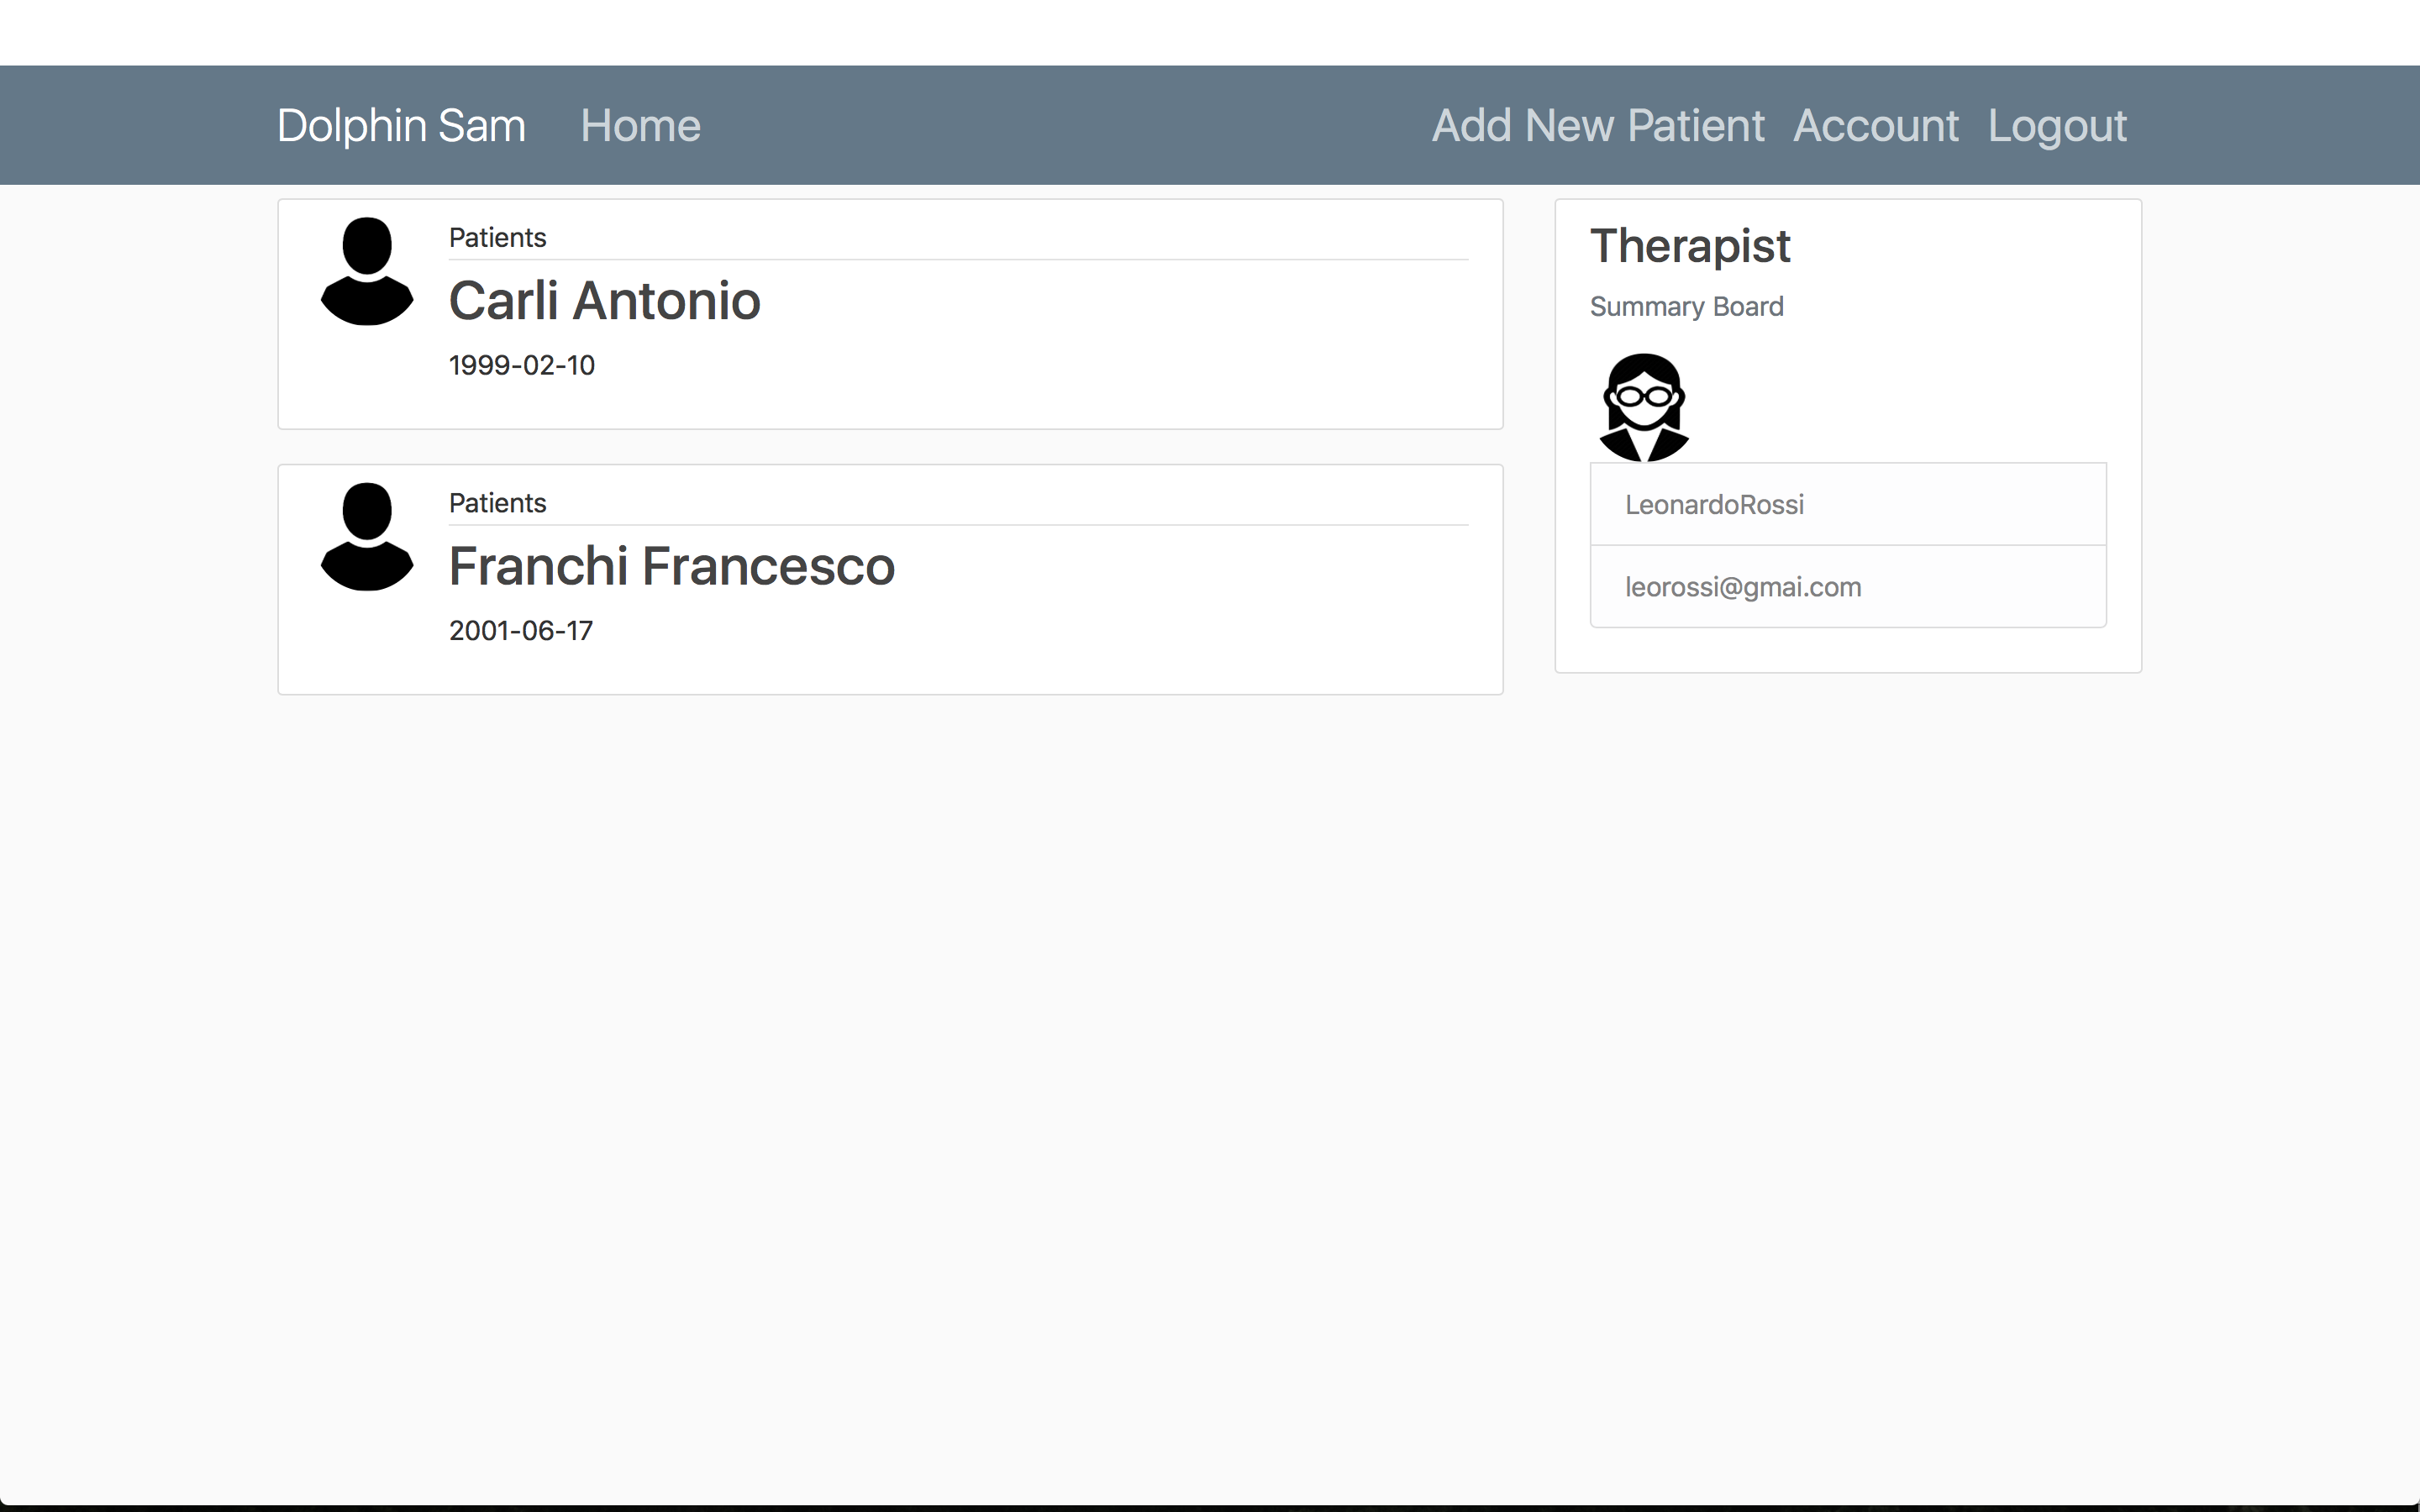
\includegraphics[width=\textwidth]{images/UX/website/4-patientsList}
	\caption{Therapist's personal home page}
	\label{fig:webPatList}
\end{figure}
In Figure \ref{fig:webPatList} is represented the website's personal page of the therapist that will be shown after a successful login authentication. Here he/she can see all his/her patients' records (note that a therapist can only manage and access records about his/her own patients), choose to add a new patient by pressing the "Add New Patient" button, edit his/her account by clicking the "Account" button and logout via the "Logout" button.

\begin{figure}[h!]
	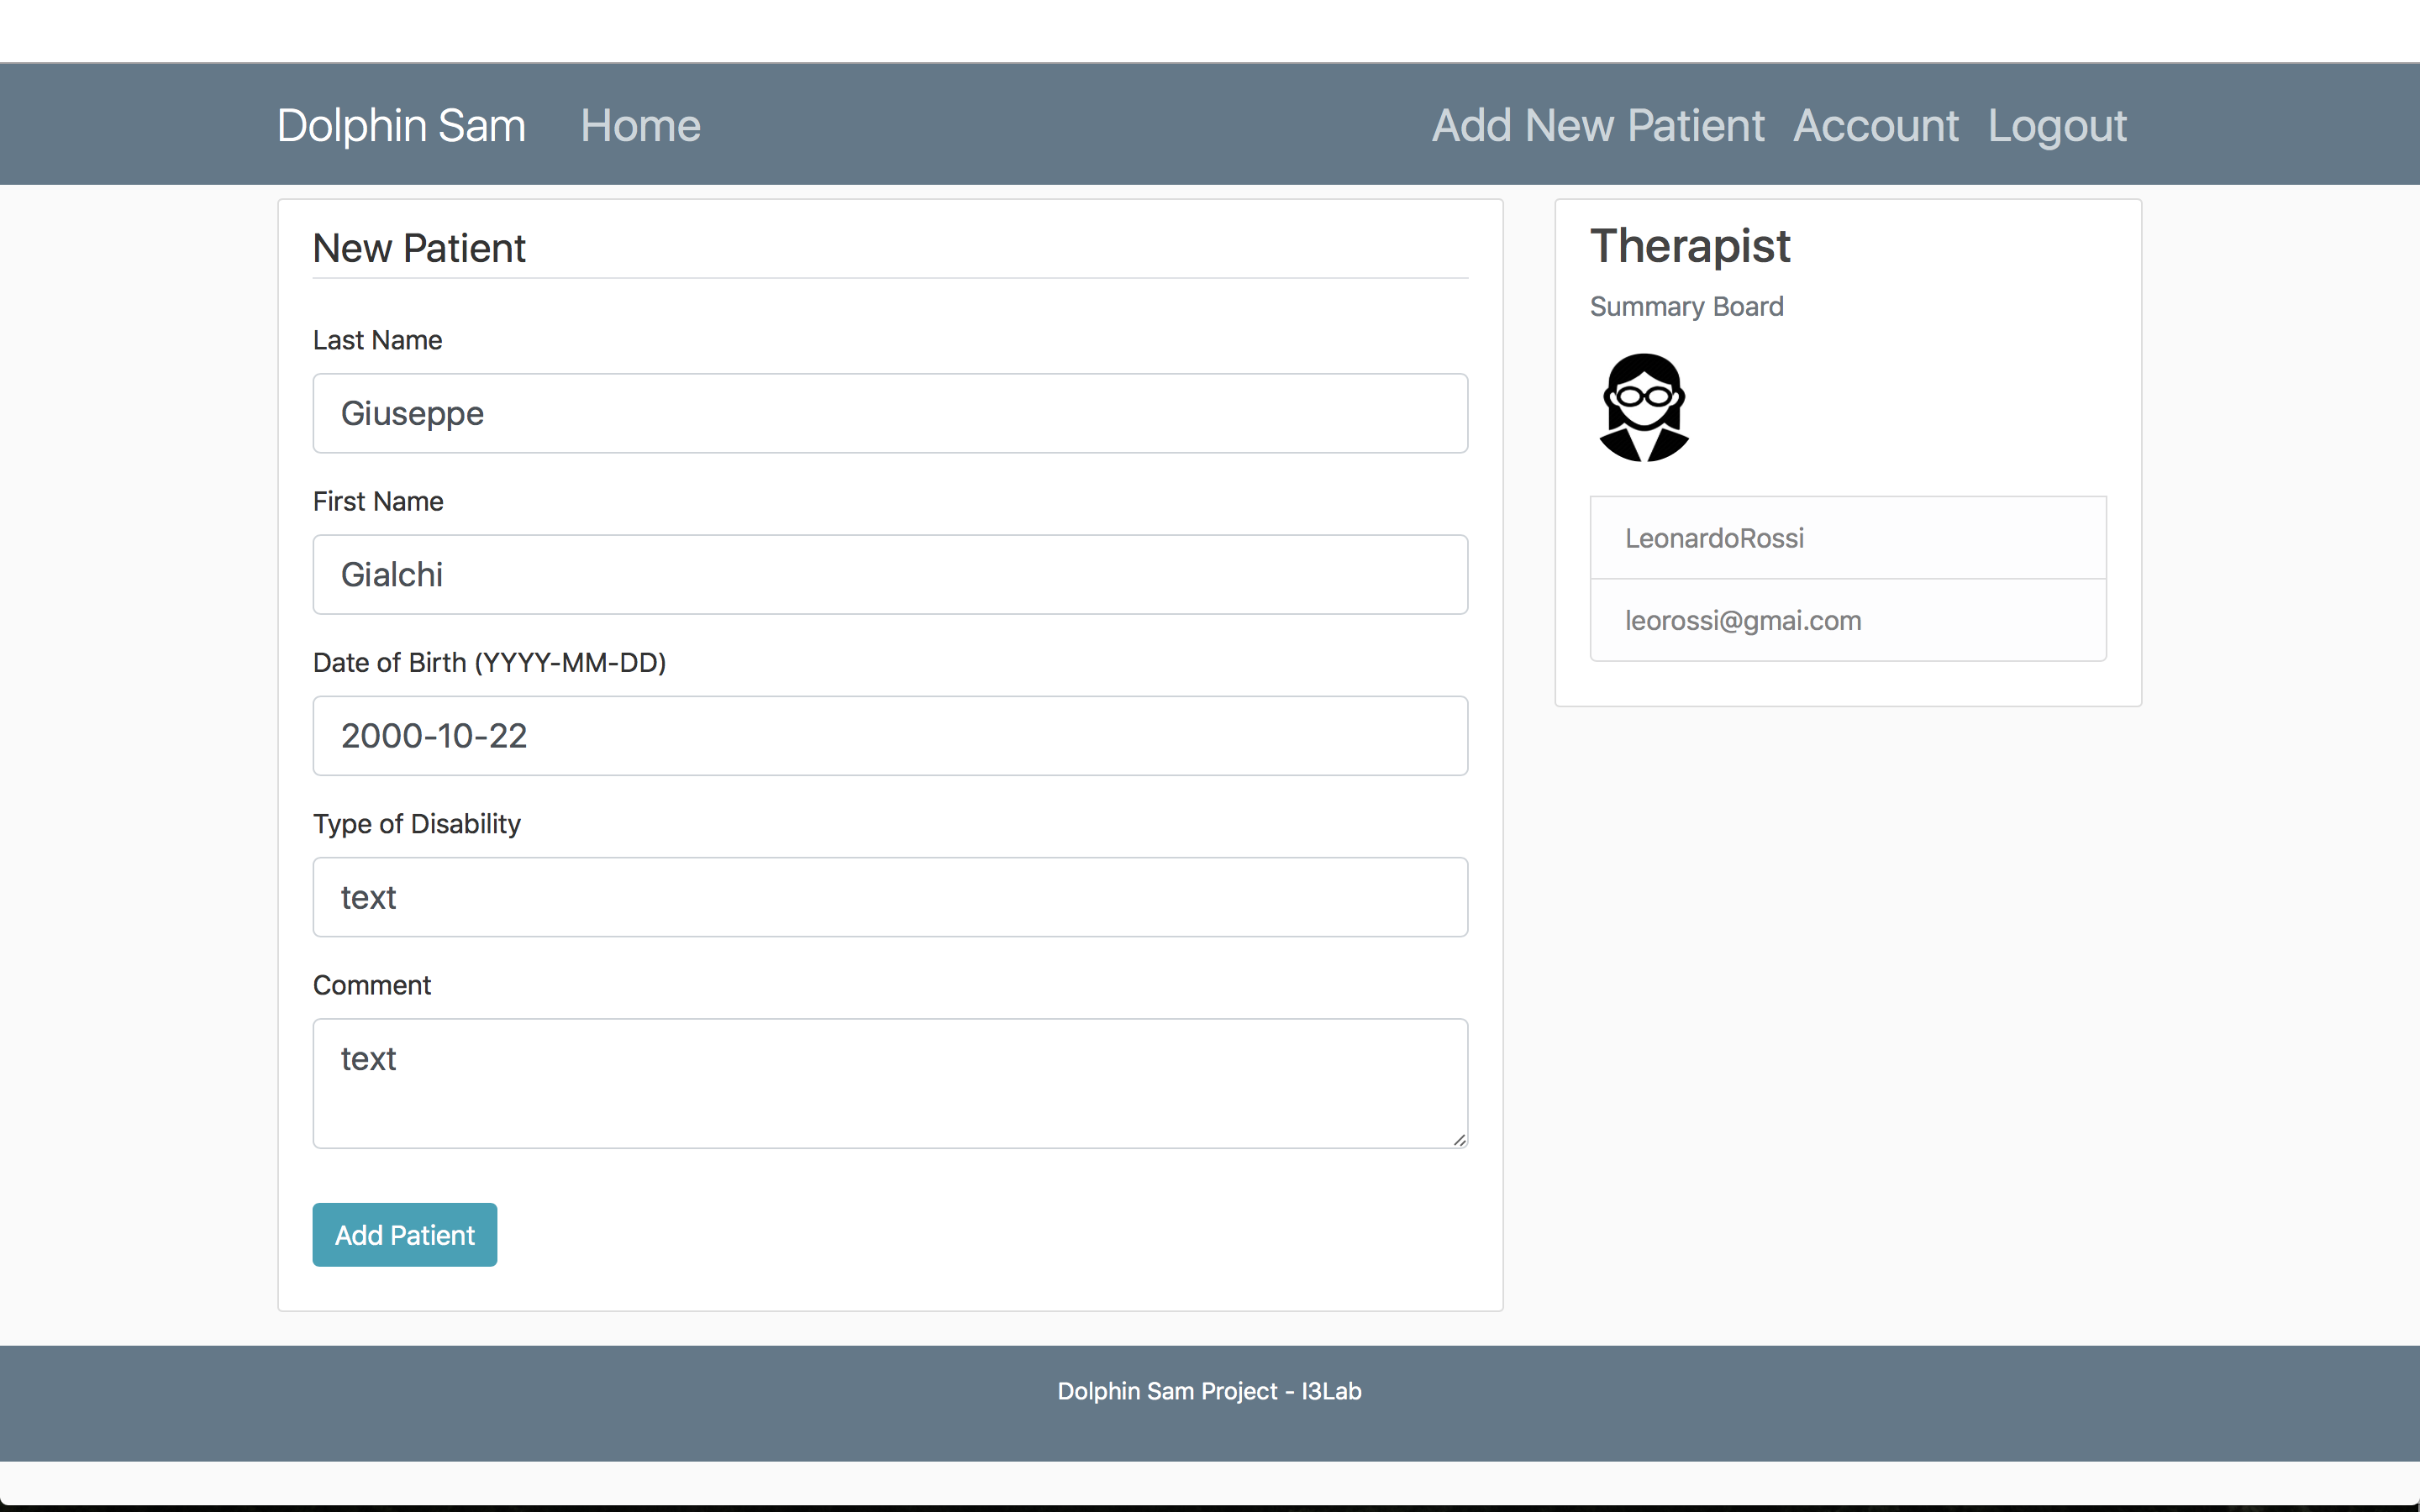
\includegraphics[width=\textwidth]{images/UX/website/6-addNewPatient}
	\caption{Add a new patient form}
	\label{fig:webAddPat}
\end{figure}
\pagebreak
In Figure  \ref{fig:webAddPat} is represented the form that will be used to collect the patient's information during the registration process brought by the therapist. When completed the new patient's record will be made persistent and added to the therapist's list of patients by clicking on the "Add Patient" button below.
\begin{figure}[h]
	\centering
	\begin{minipage}[b]{0.49\textwidth}
		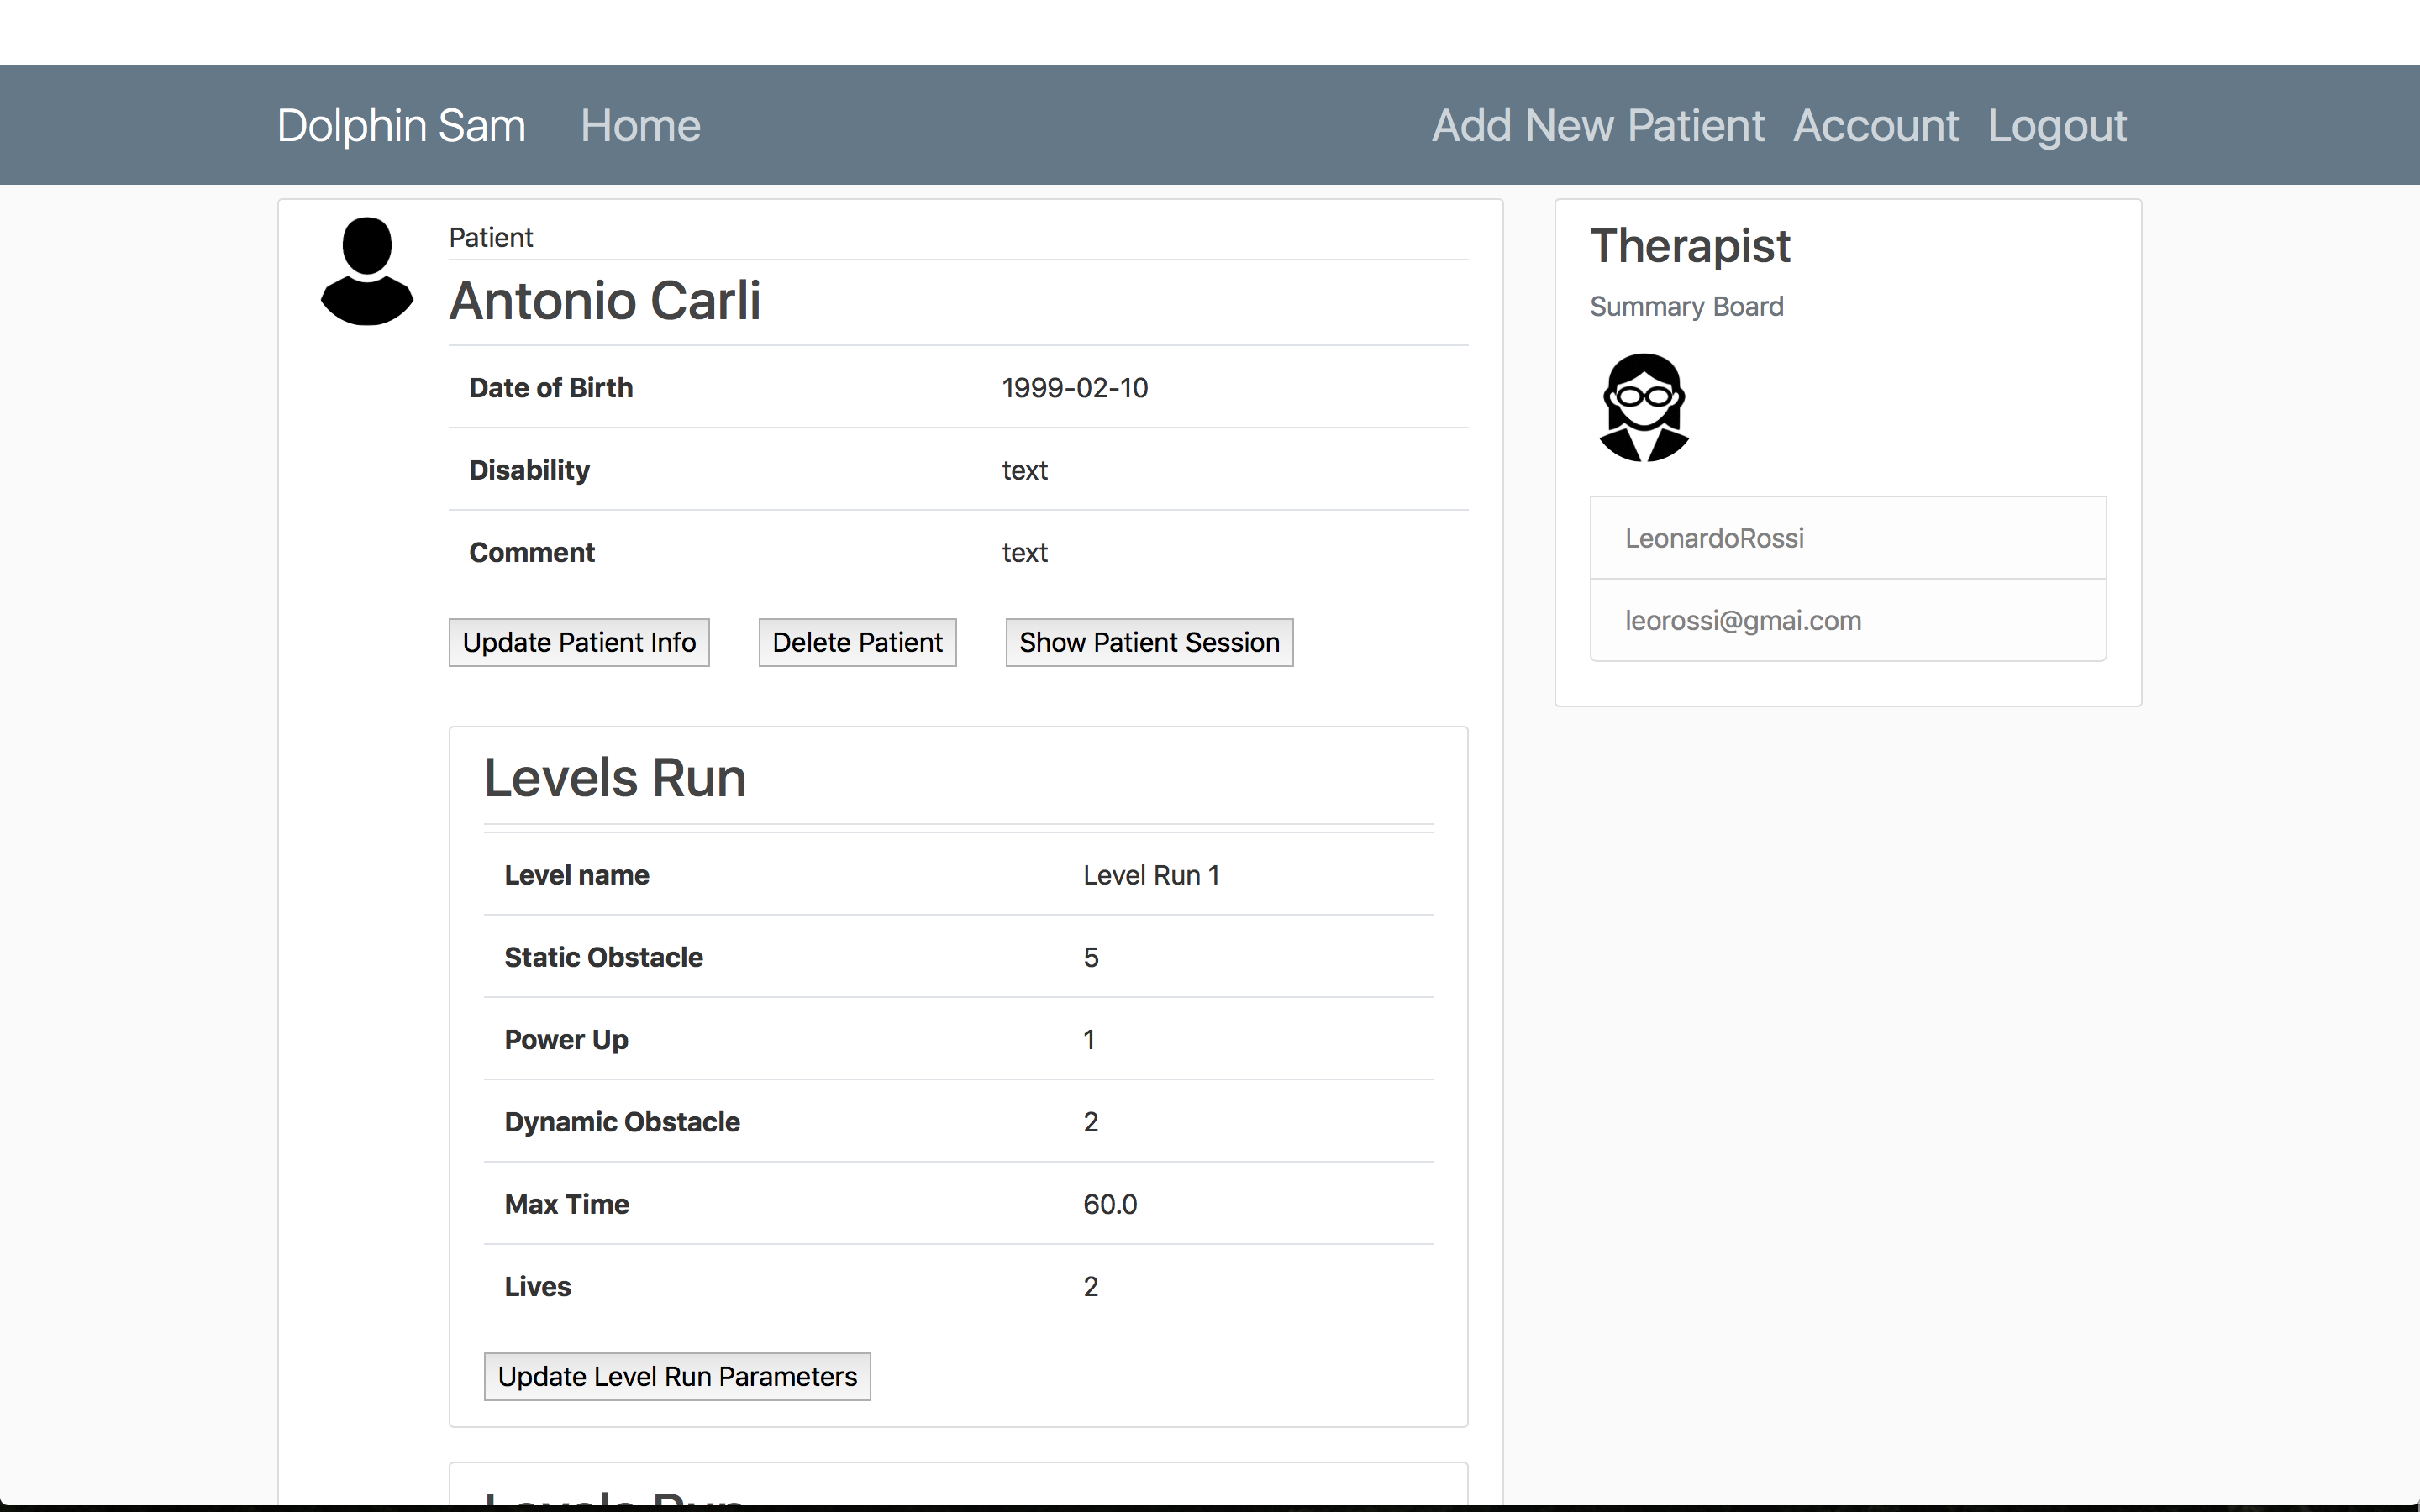
\includegraphics[width=\textwidth]{images/UX/website/7-detailPatient}
		\caption{Patient's parameters for the Run activity}
		\label{fig:webPatPar1}
	\end{minipage}
	\begin{minipage}[b]{0.49\textwidth}
		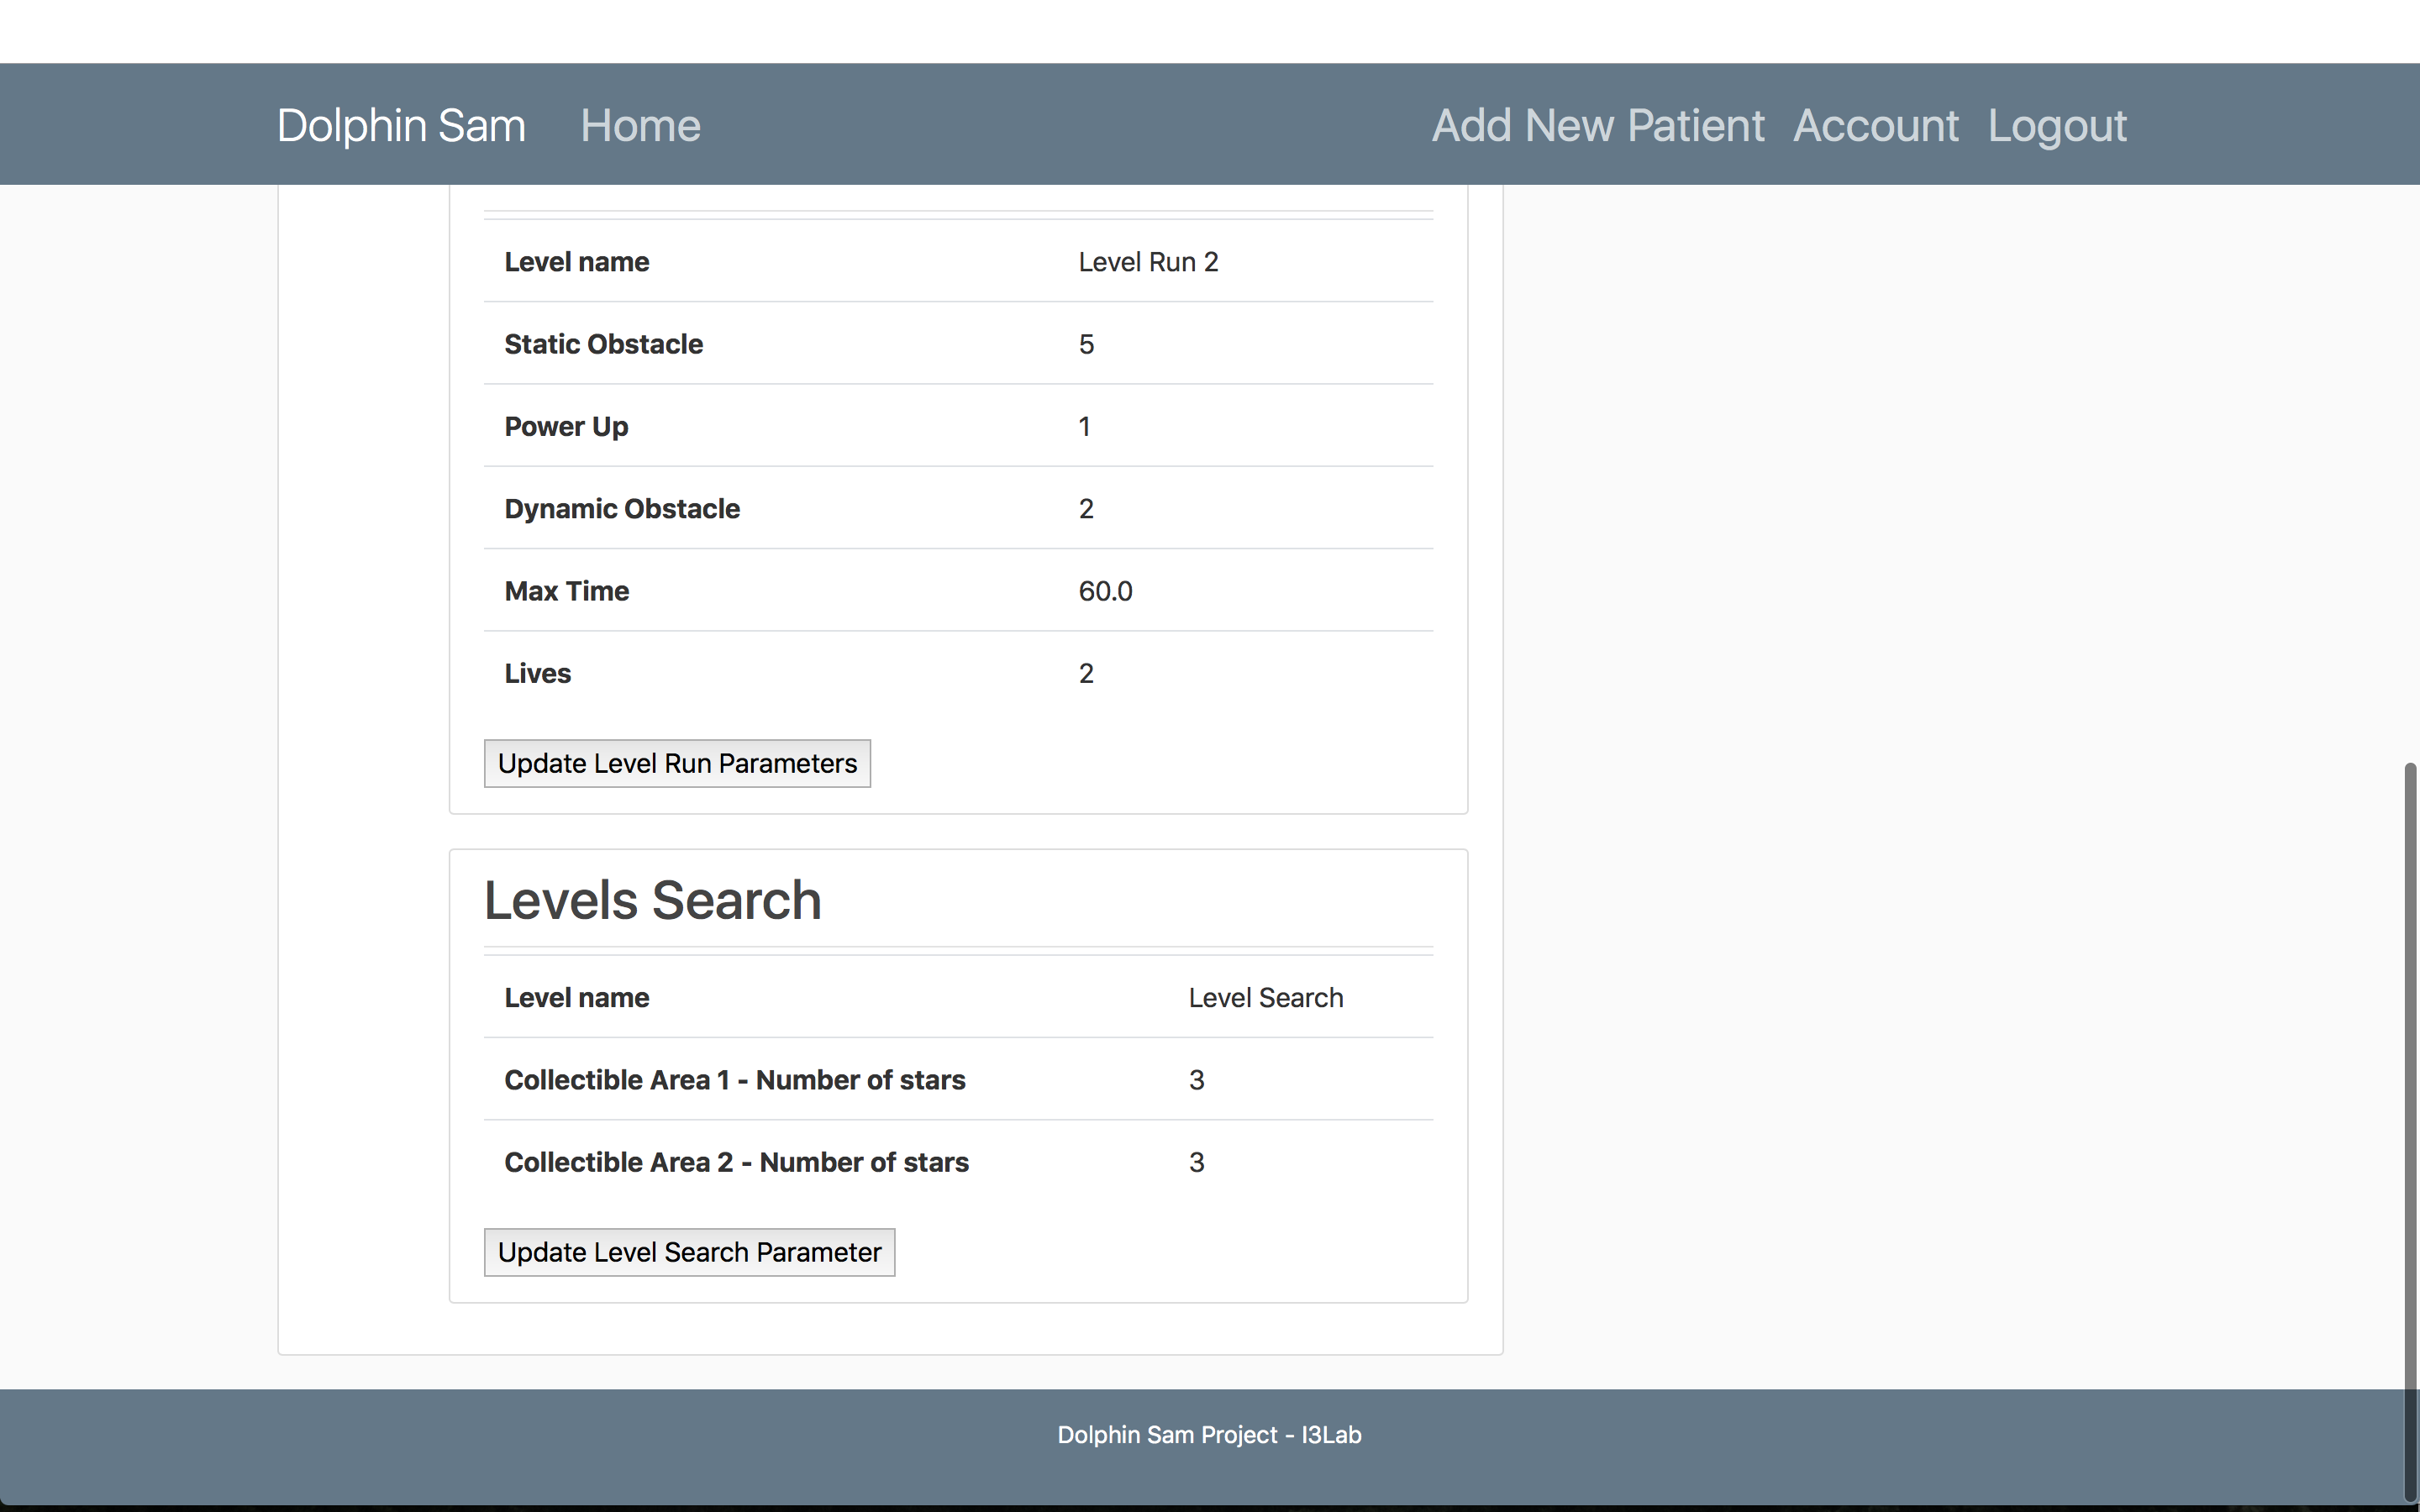
\includegraphics[width=\textwidth]{images/UX/website/8-detailPatient}
		\caption{Patient's parameters for the Search activity}
		\label{fig:webPatPar2}
	\end{minipage}
\end{figure}

By selecting a patient from the list (Figure  \ref{fig:webPatList})  the therapist is redirected to the patient's details page (Figure \ref{fig:webPatPar1}, \ref{fig:webPatPar2}) which contains the patient's information and the parameters that will be used to set the different levels of difficulty for the various activities. Those parameters can be updated by selecting the respective "Update" button below in order to customize the activities for the specific patient starting from the next session.

%\begin{figure}[h]
%	\centering
%	\begin{minipage}[b]{0.4\textwidth}
%		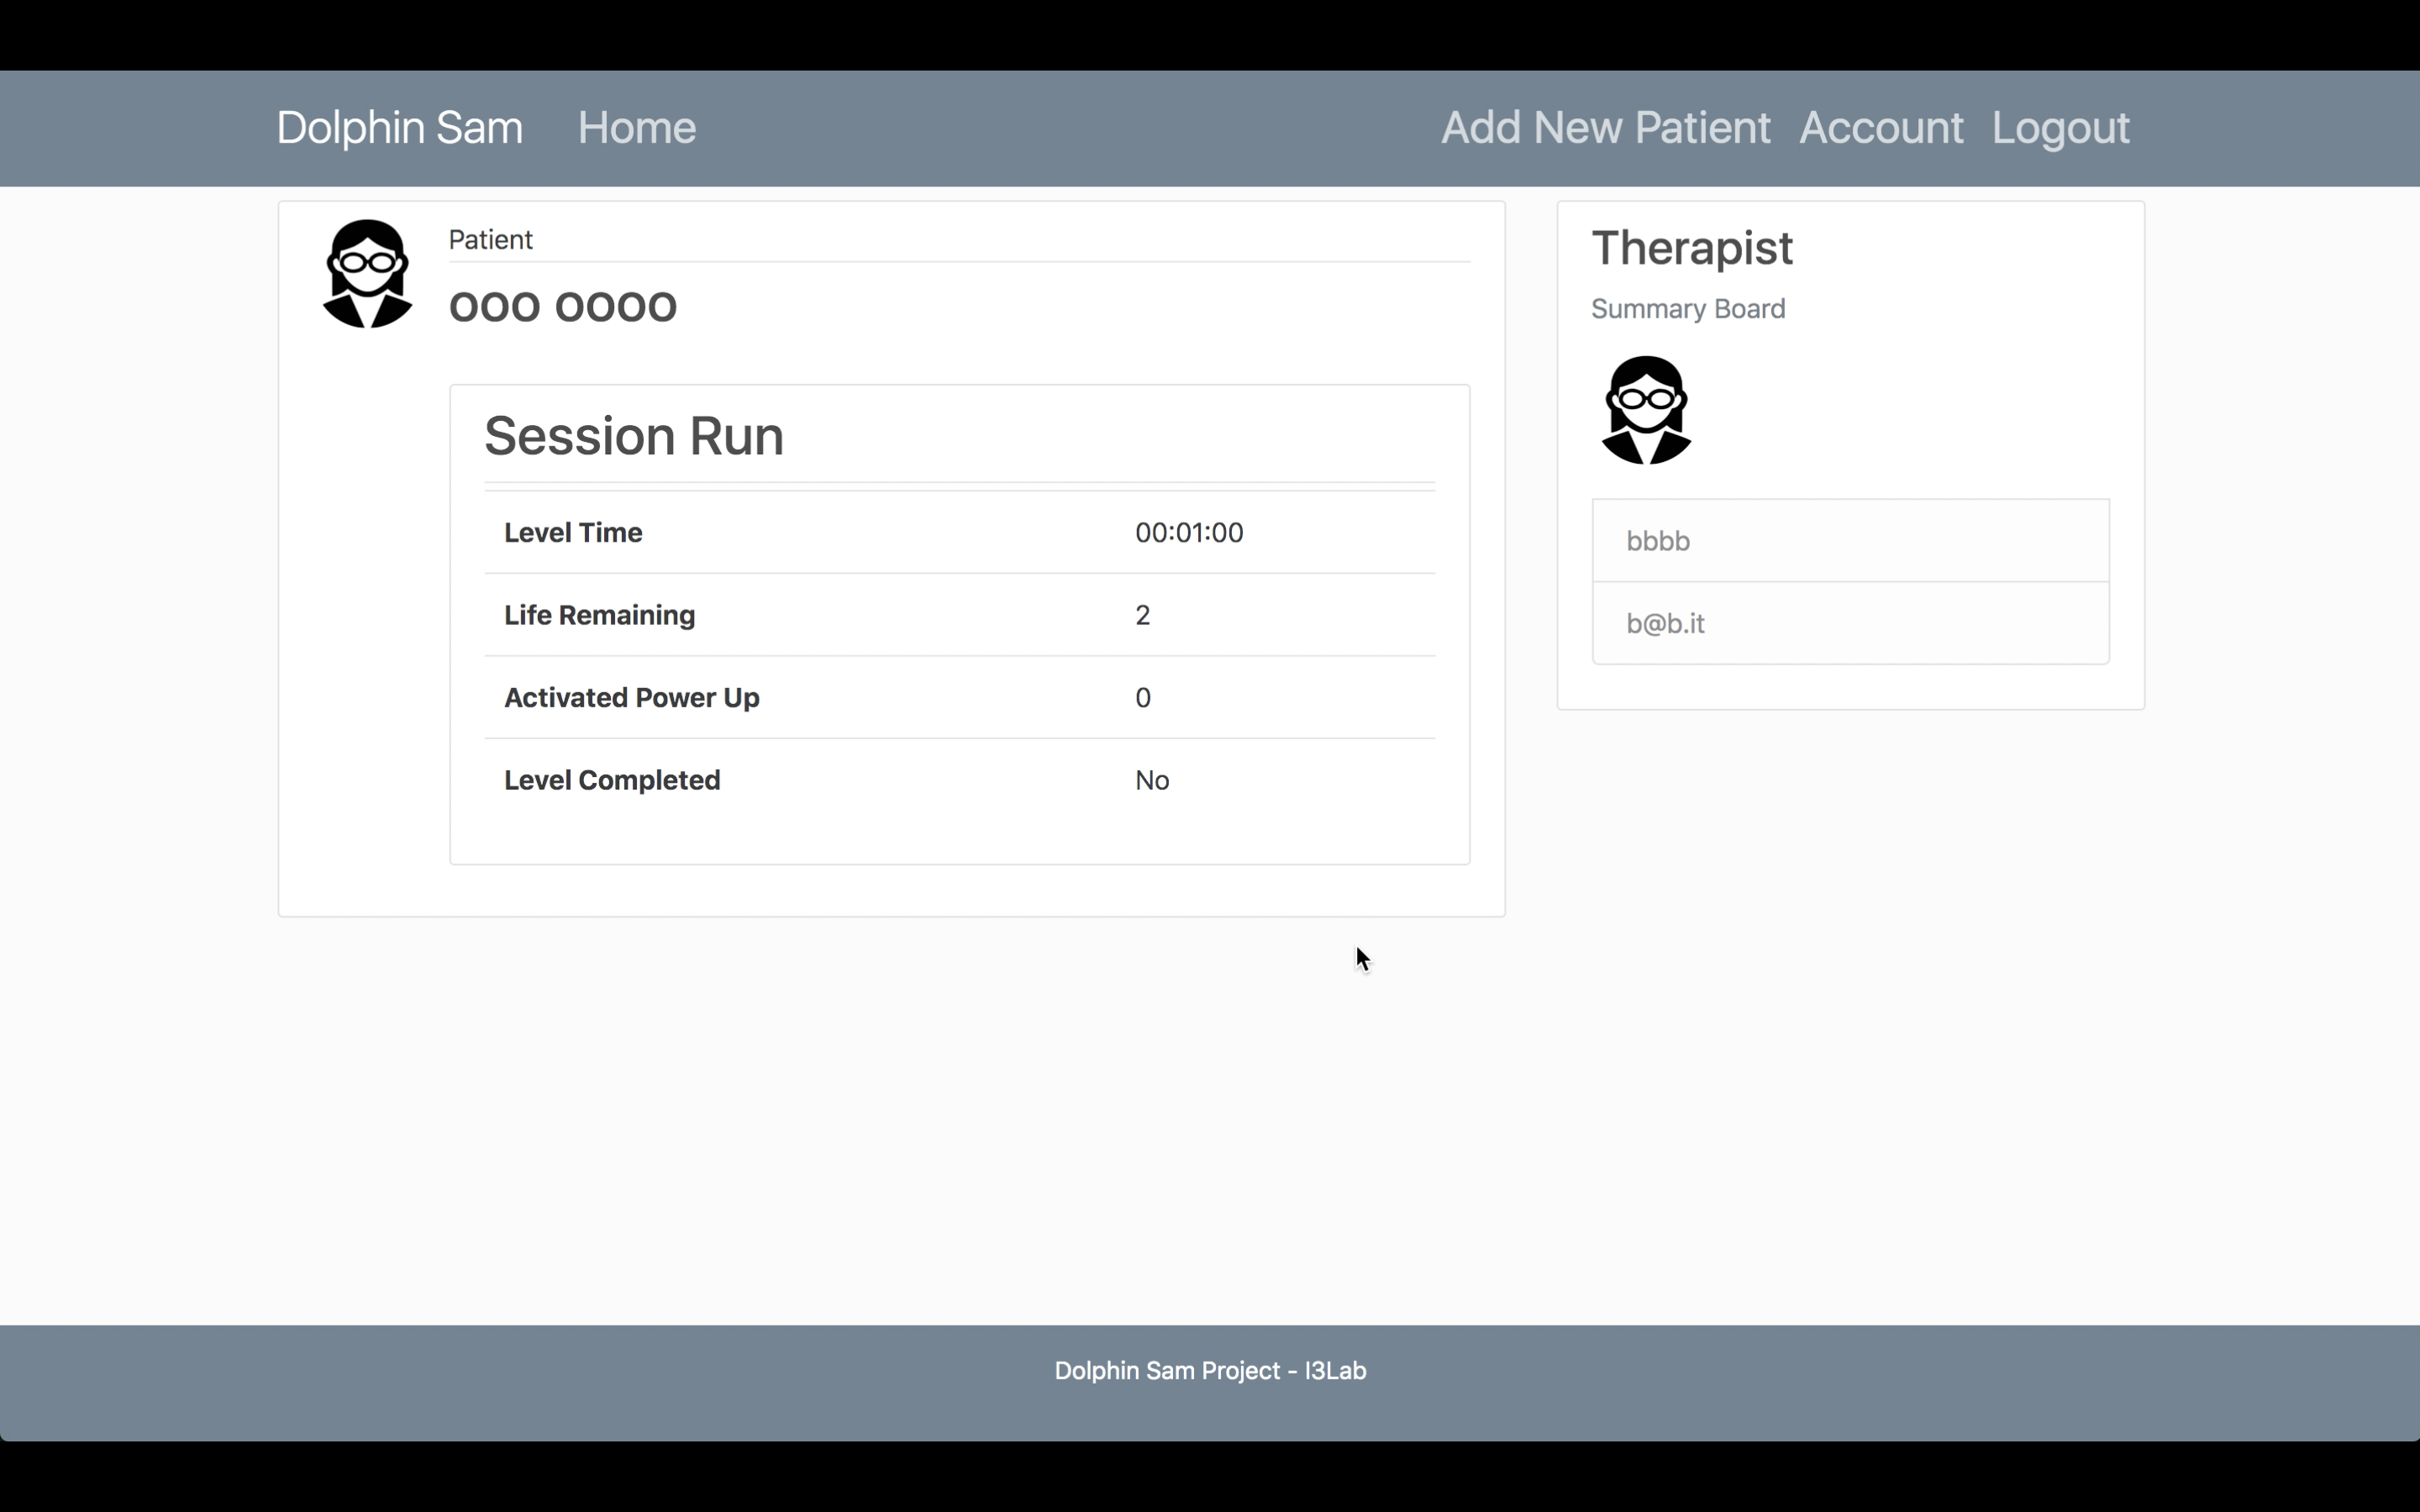
\includegraphics[width=\textwidth]{images/UX/website/11-runAnal}
%		\caption{Session data for Dolphin Run activity}
%		\label{fig:webAnalRun}
%	\end{minipage}
%	\hfill
%	\begin{minipage}[b]{0.4\textwidth}
%		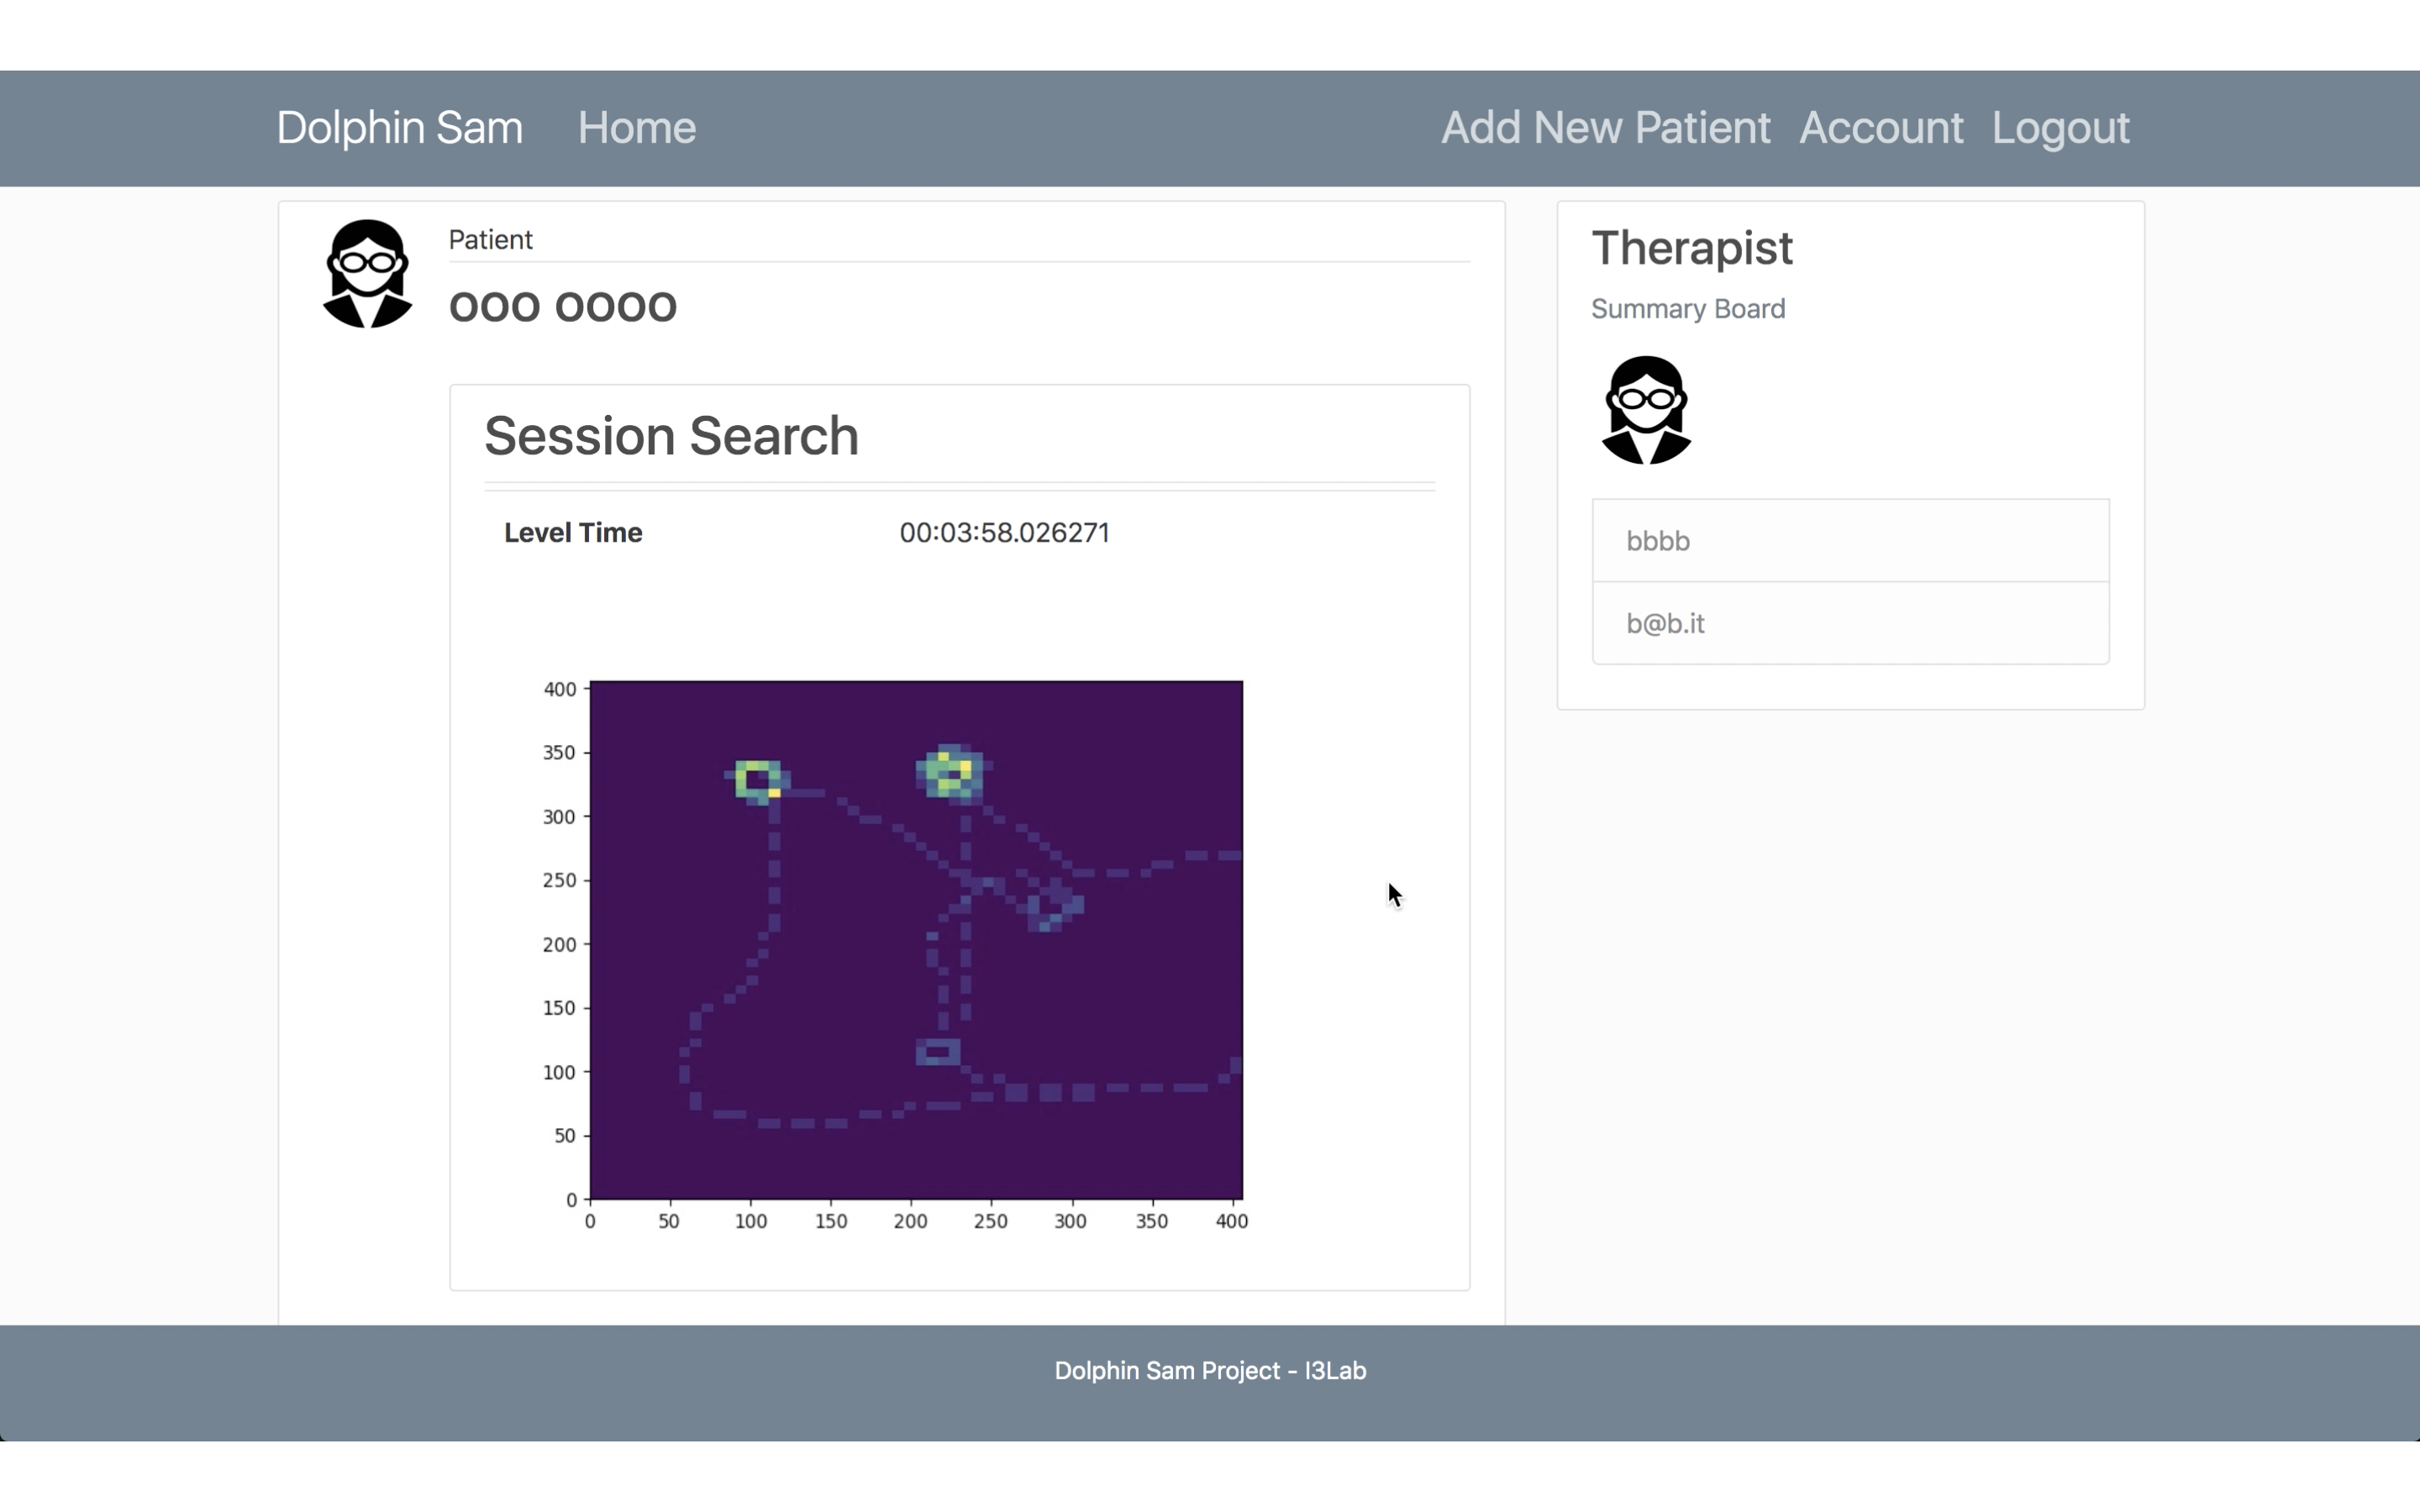
\includegraphics[width=\textwidth]{images/UX/website/12-searchAnal}
%		\caption{Session data for Dolphin Search activity}
%		\label{fig:webAnalSearch}
%	\end{minipage}
%\end{figure}

By clicking on the "Show Patient Session" button in a patient's detail page the therapist is able to see the data regarding all the session performed by the patient during the Dolphin Run activity (Figure \ref{fig:webAnalRun}) and the Dolphin Search activity (Figure \ref{fig:webAnalSearch}).



\subsection{Unity client}
\begin{figure}[h!]
	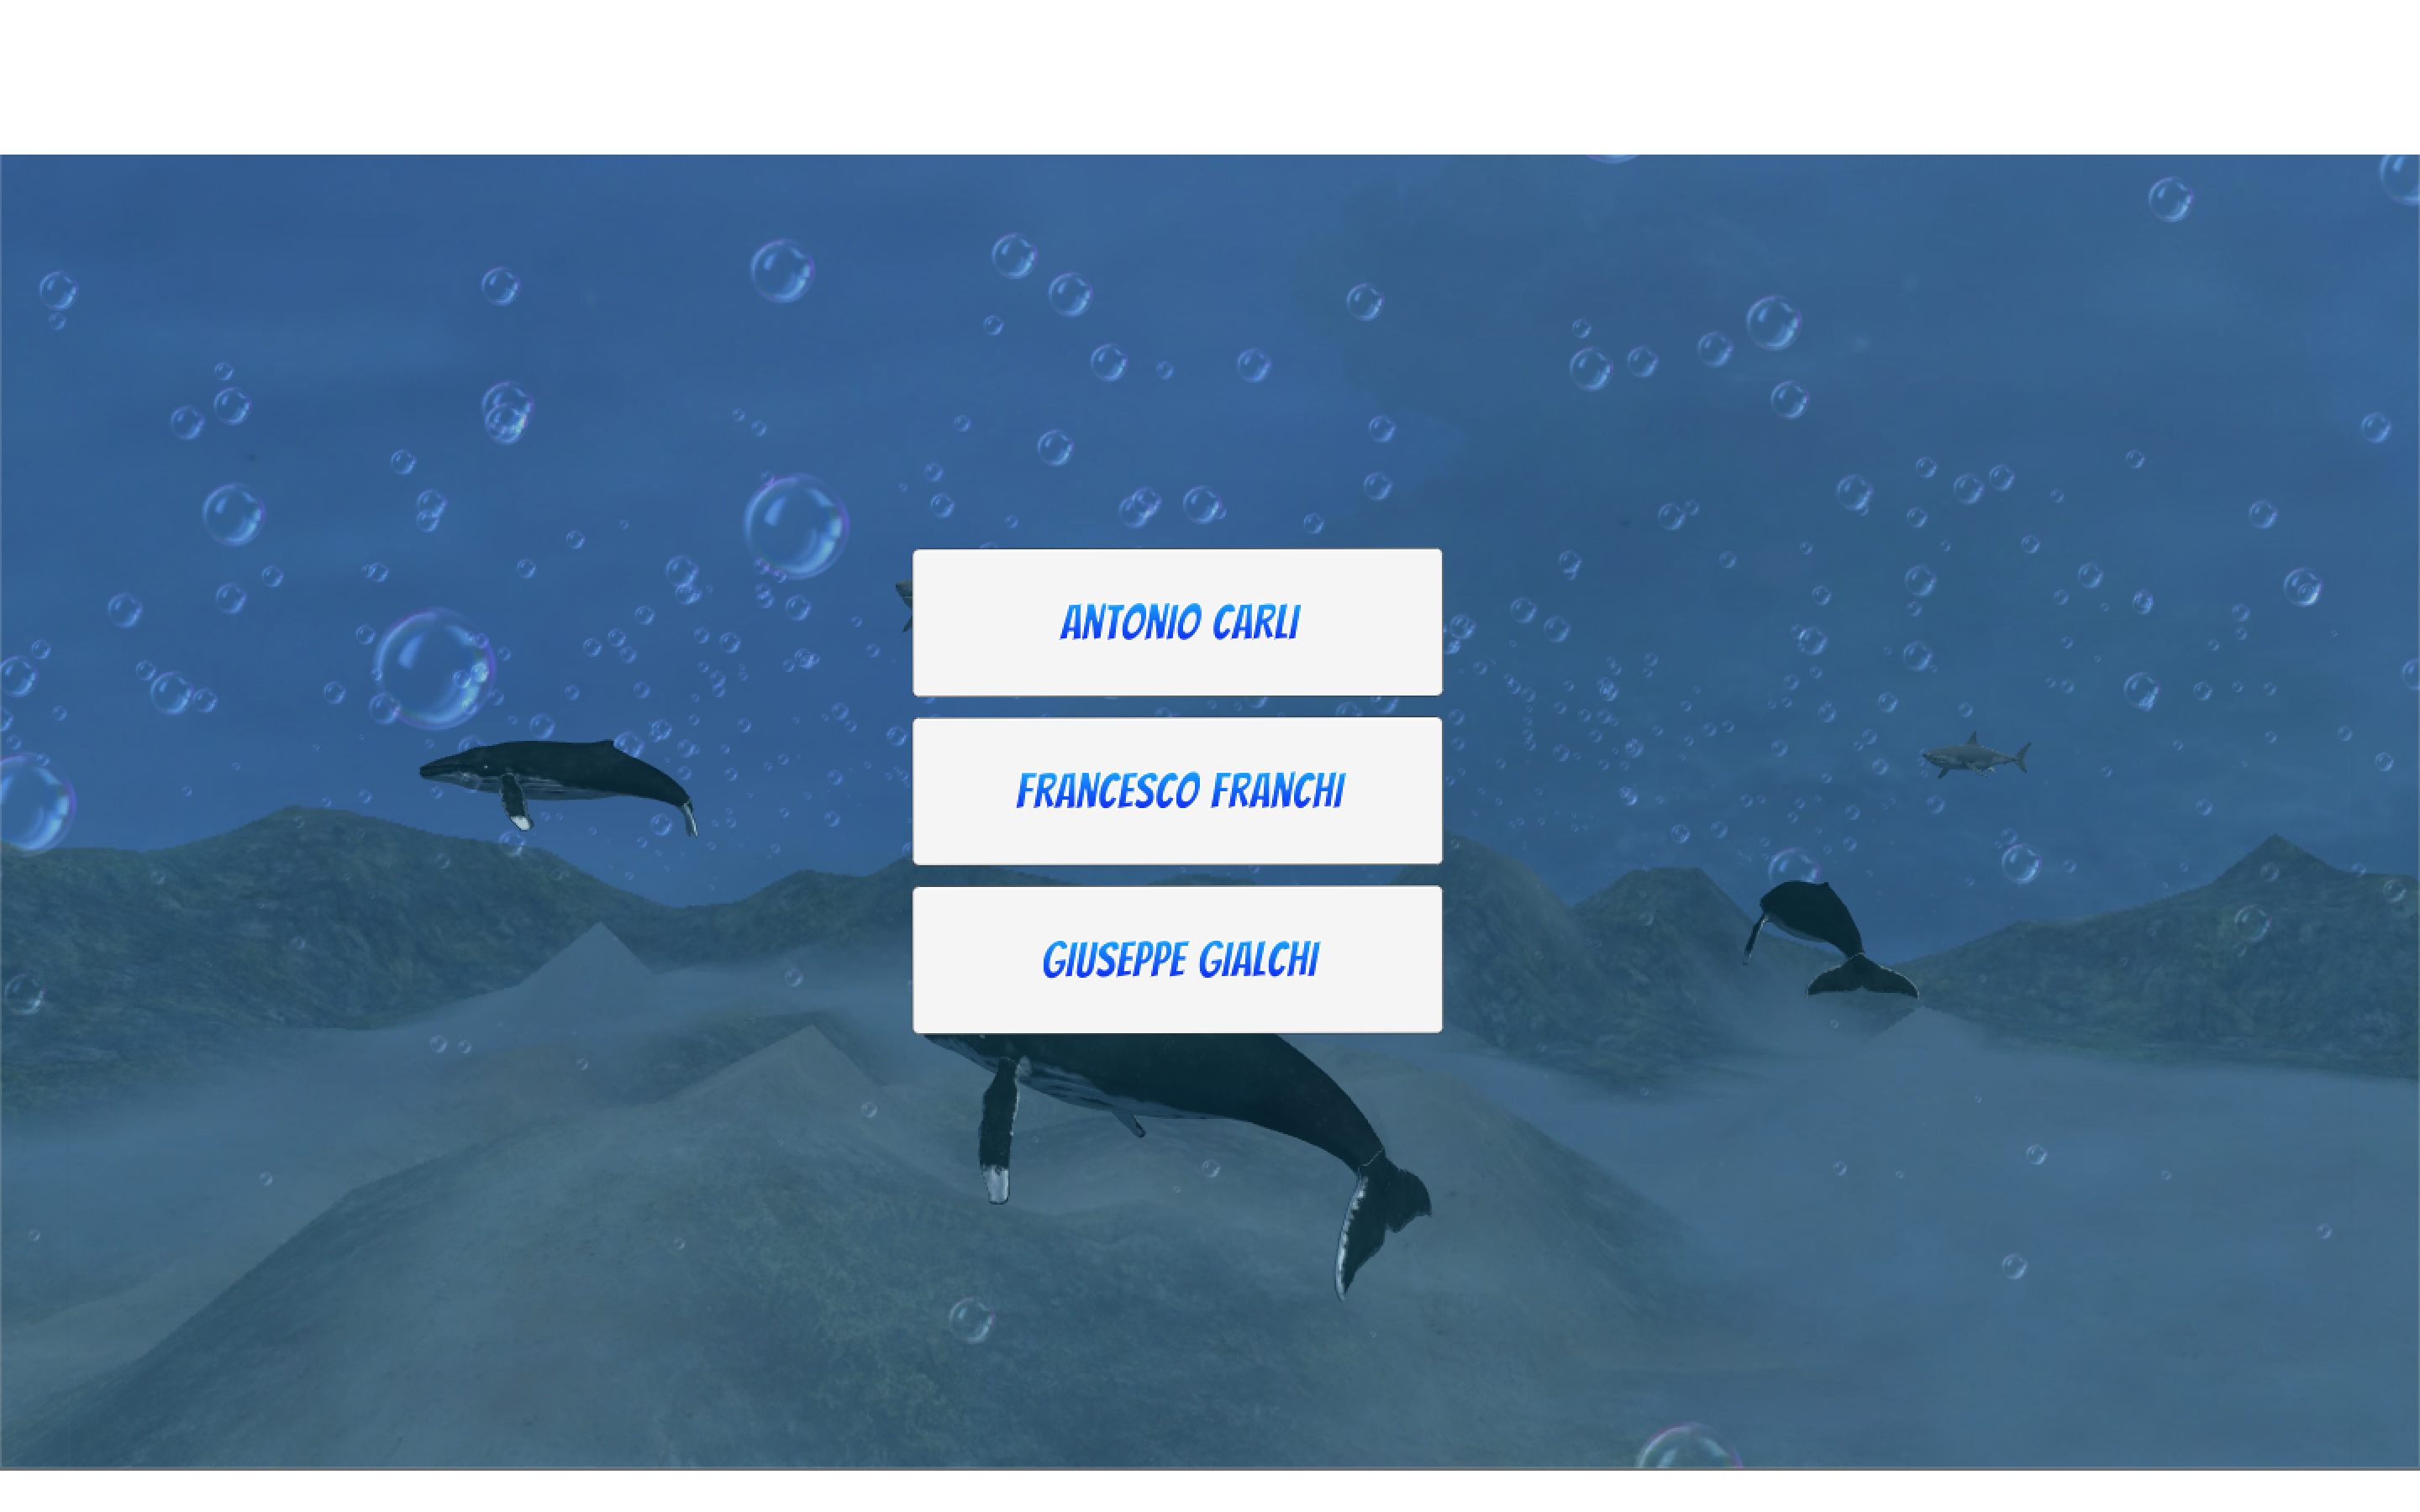
\includegraphics[width=\textwidth]{images/UX/unity/menu/3-patientList}
	\caption{Therapist's patient list}
	\label{fig:unityPatList}
\end{figure}

Once the game is started and the therapist is logged in, his/her patients' list is shown (Figure \ref{fig:unityPatList}) and the patient that will perform the session has to be selected using the mouse.
\pagebreak
\begin{figure}[h!]
	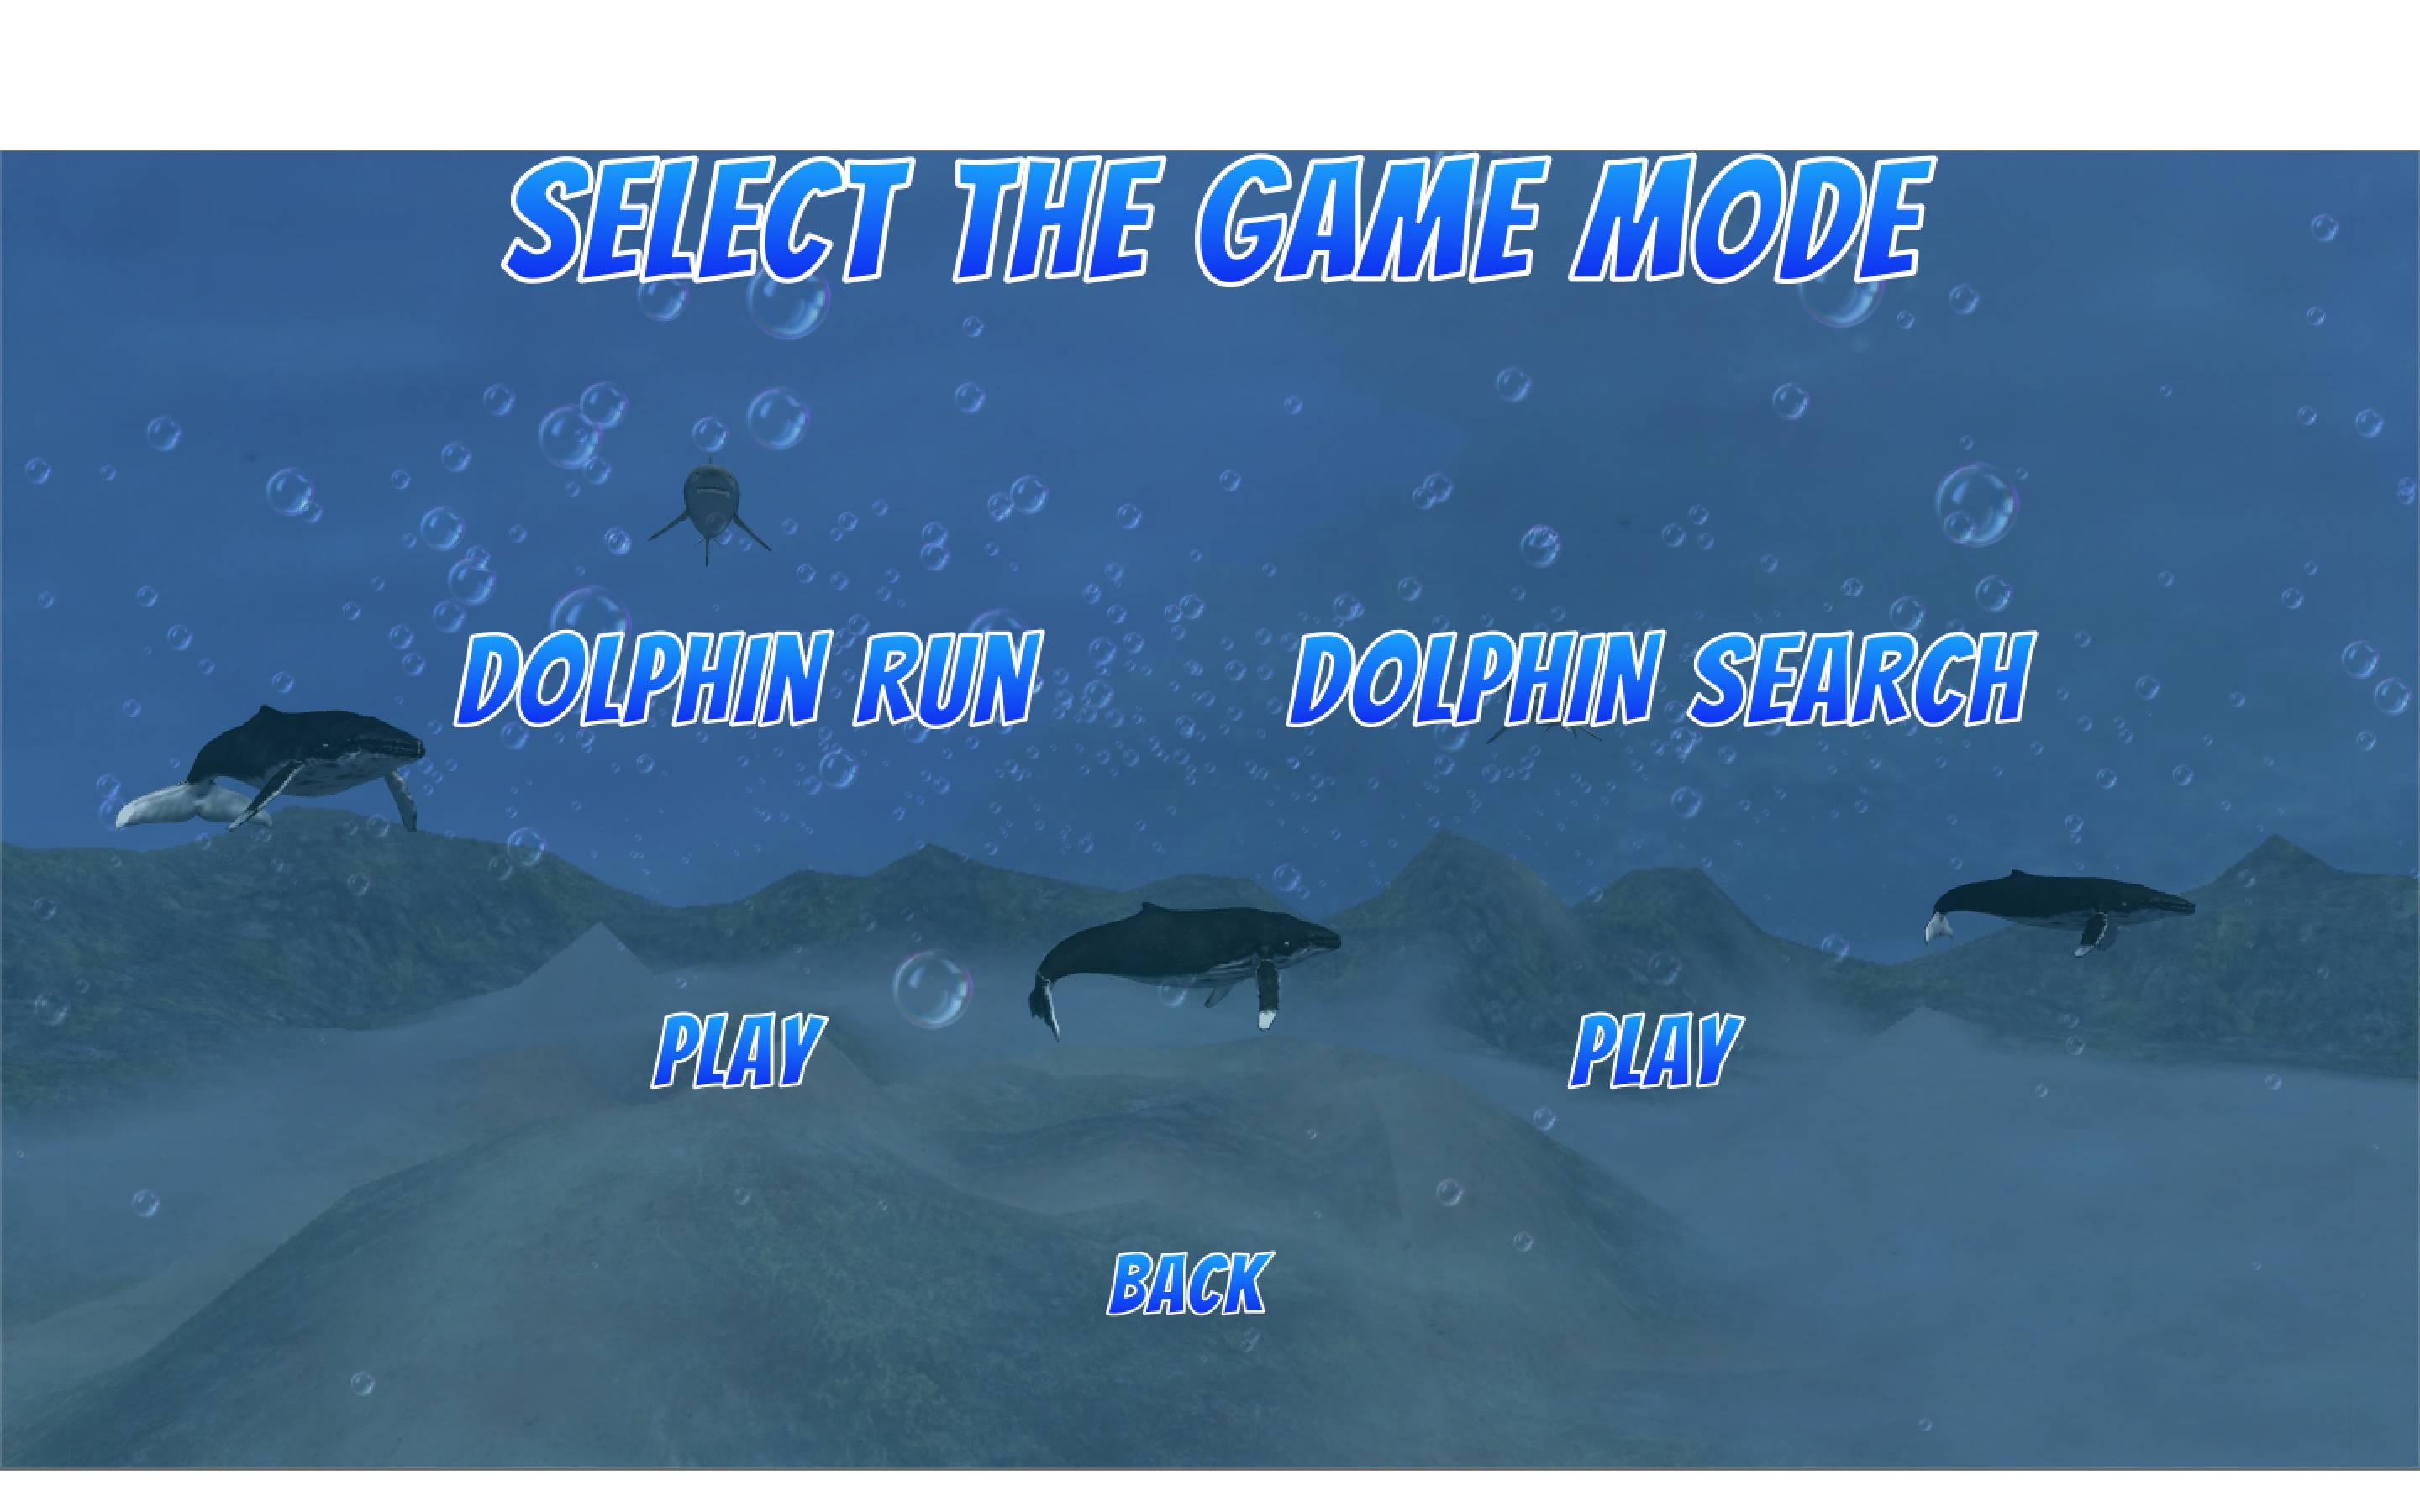
\includegraphics[width=\textwidth]{images/UX/unity/menu/4-modeSelection}
	\caption{Session's mode selection}
	\label{fig:unityModSel}
\end{figure}

After selecting a patient there will be asked to select which one of the activities (Dolphin run or Dolphin Search) will be played in the next session, still using the mouse. (Figure \ref{fig:unityModSel}).

\begin{figure}[h!]
	\centering
	\begin{minipage}[b]{0.49\textwidth}
		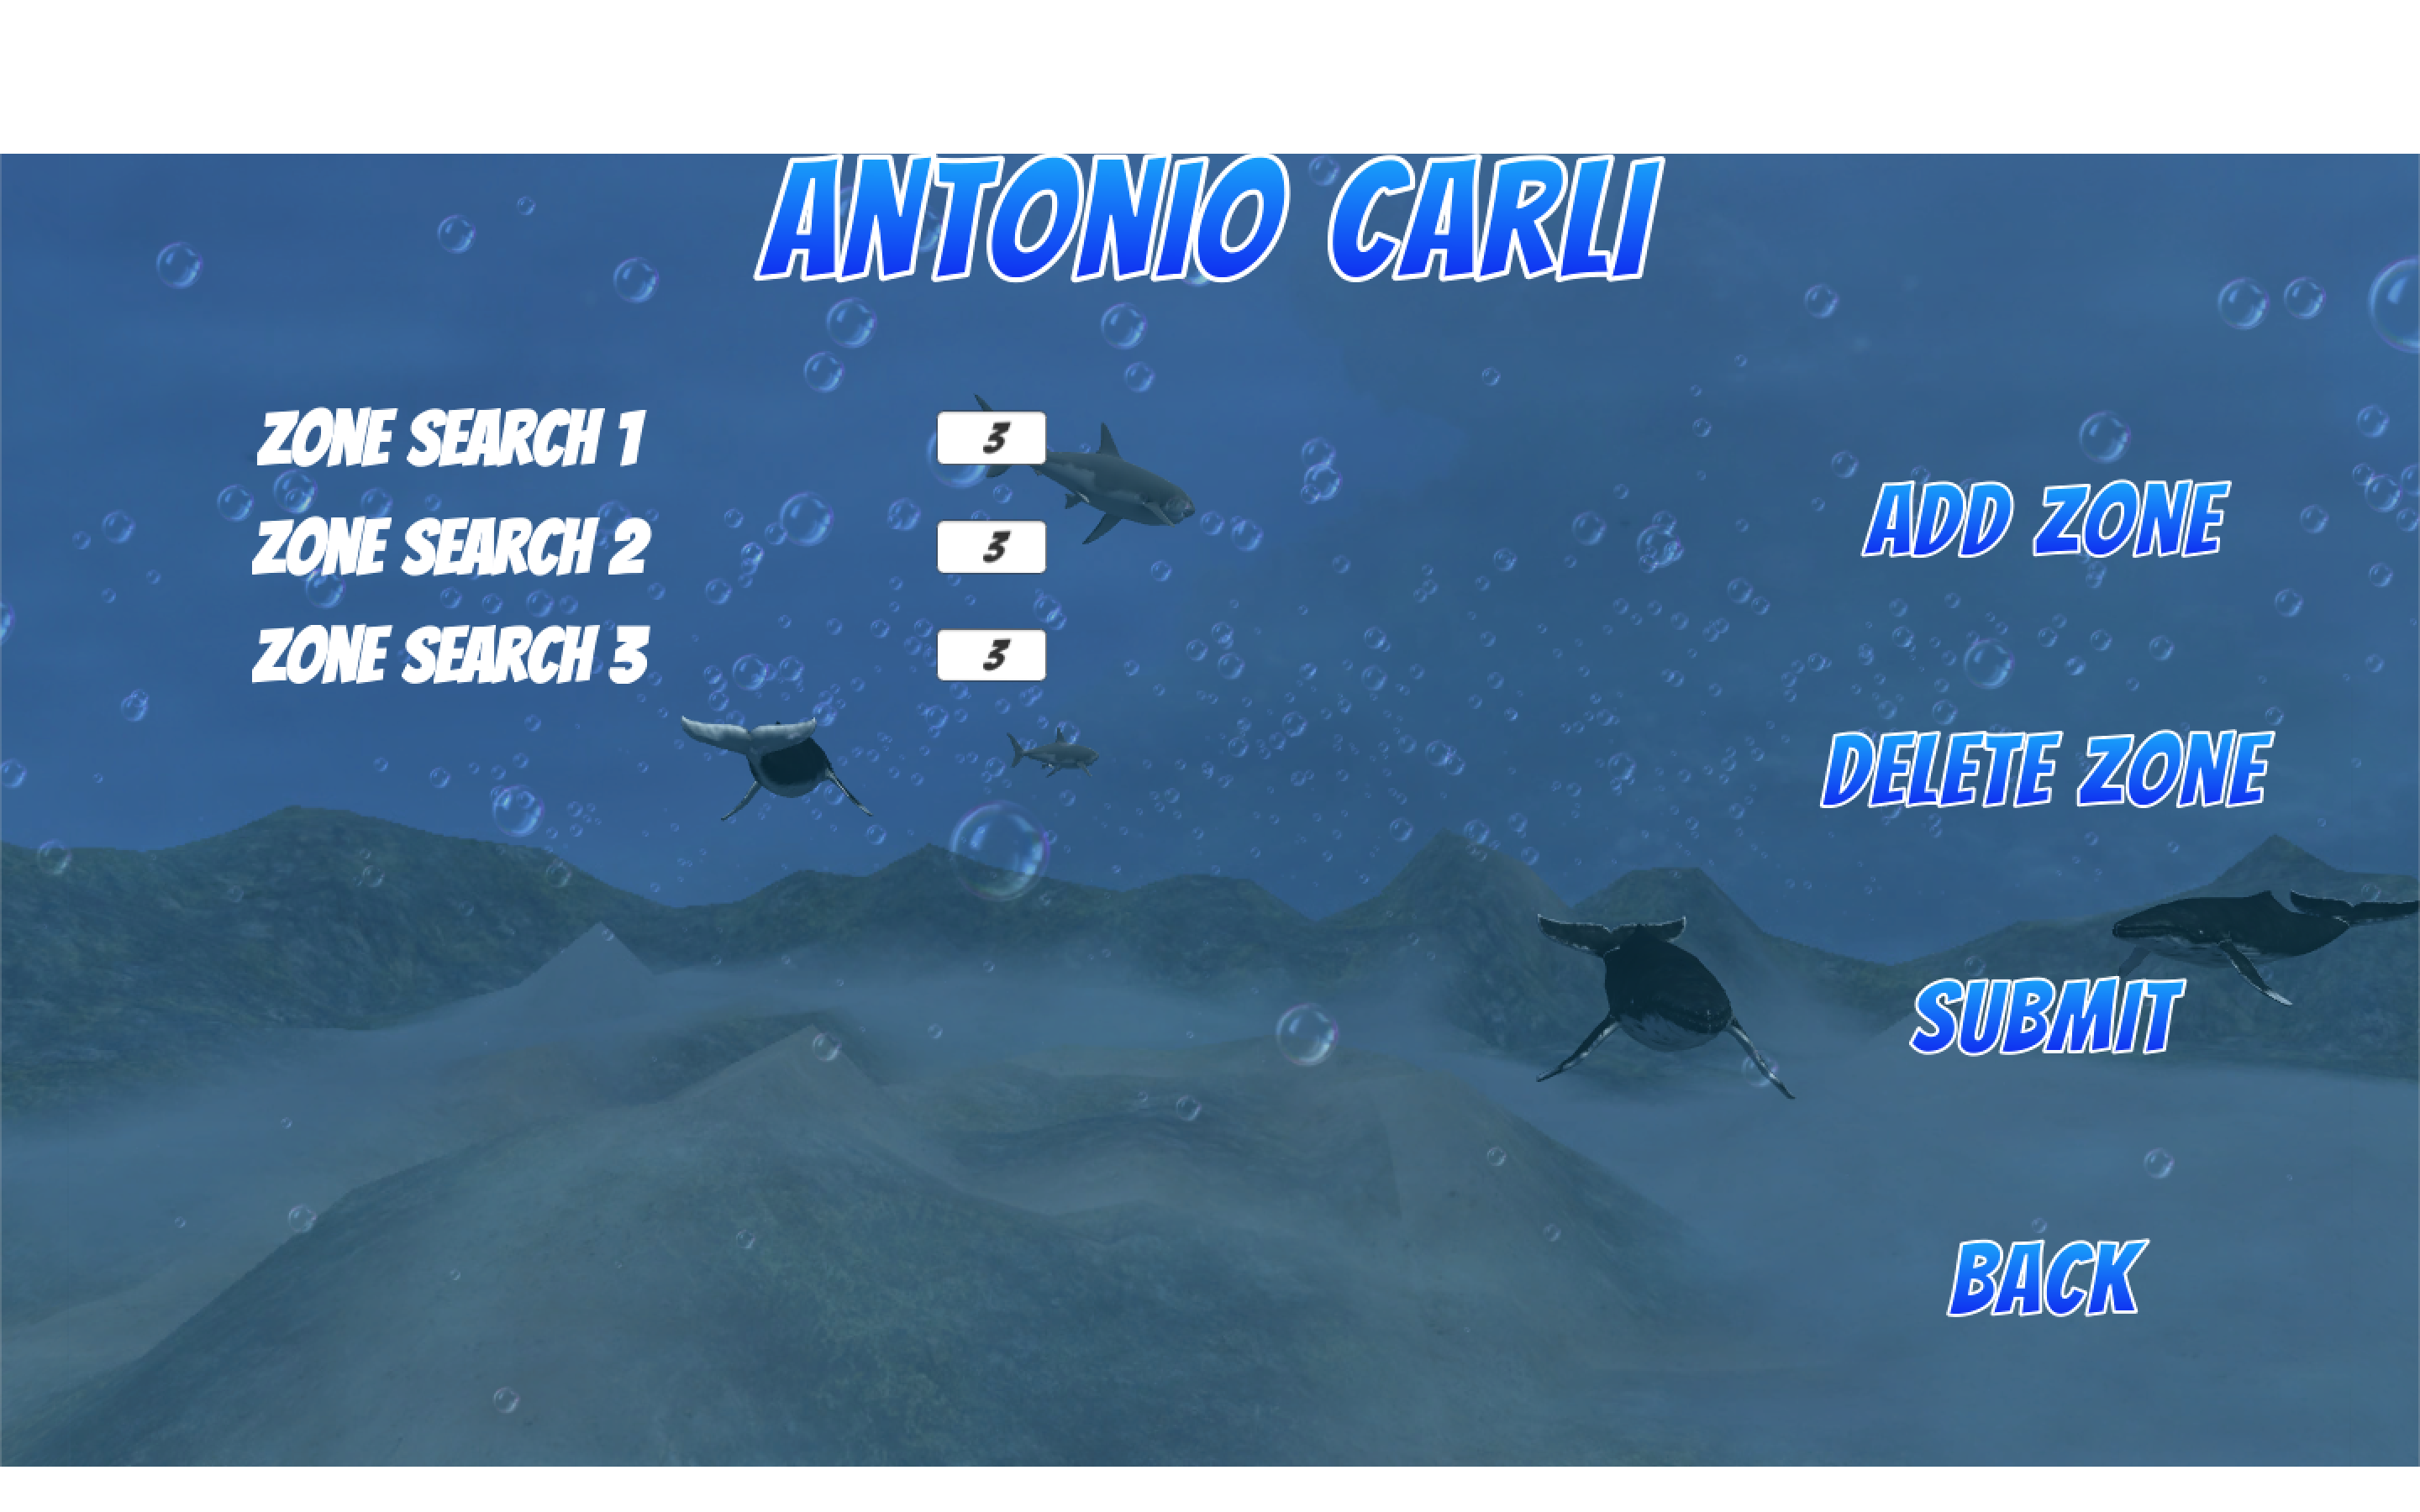
\includegraphics[width=\textwidth]{images/UX/unity/menu/5-search1}
		\caption{Parameters settings for Dolphin Run }
		\label{fig:unityParamRun}
	\end{minipage}
	\begin{minipage}[b]{0.49\textwidth}
		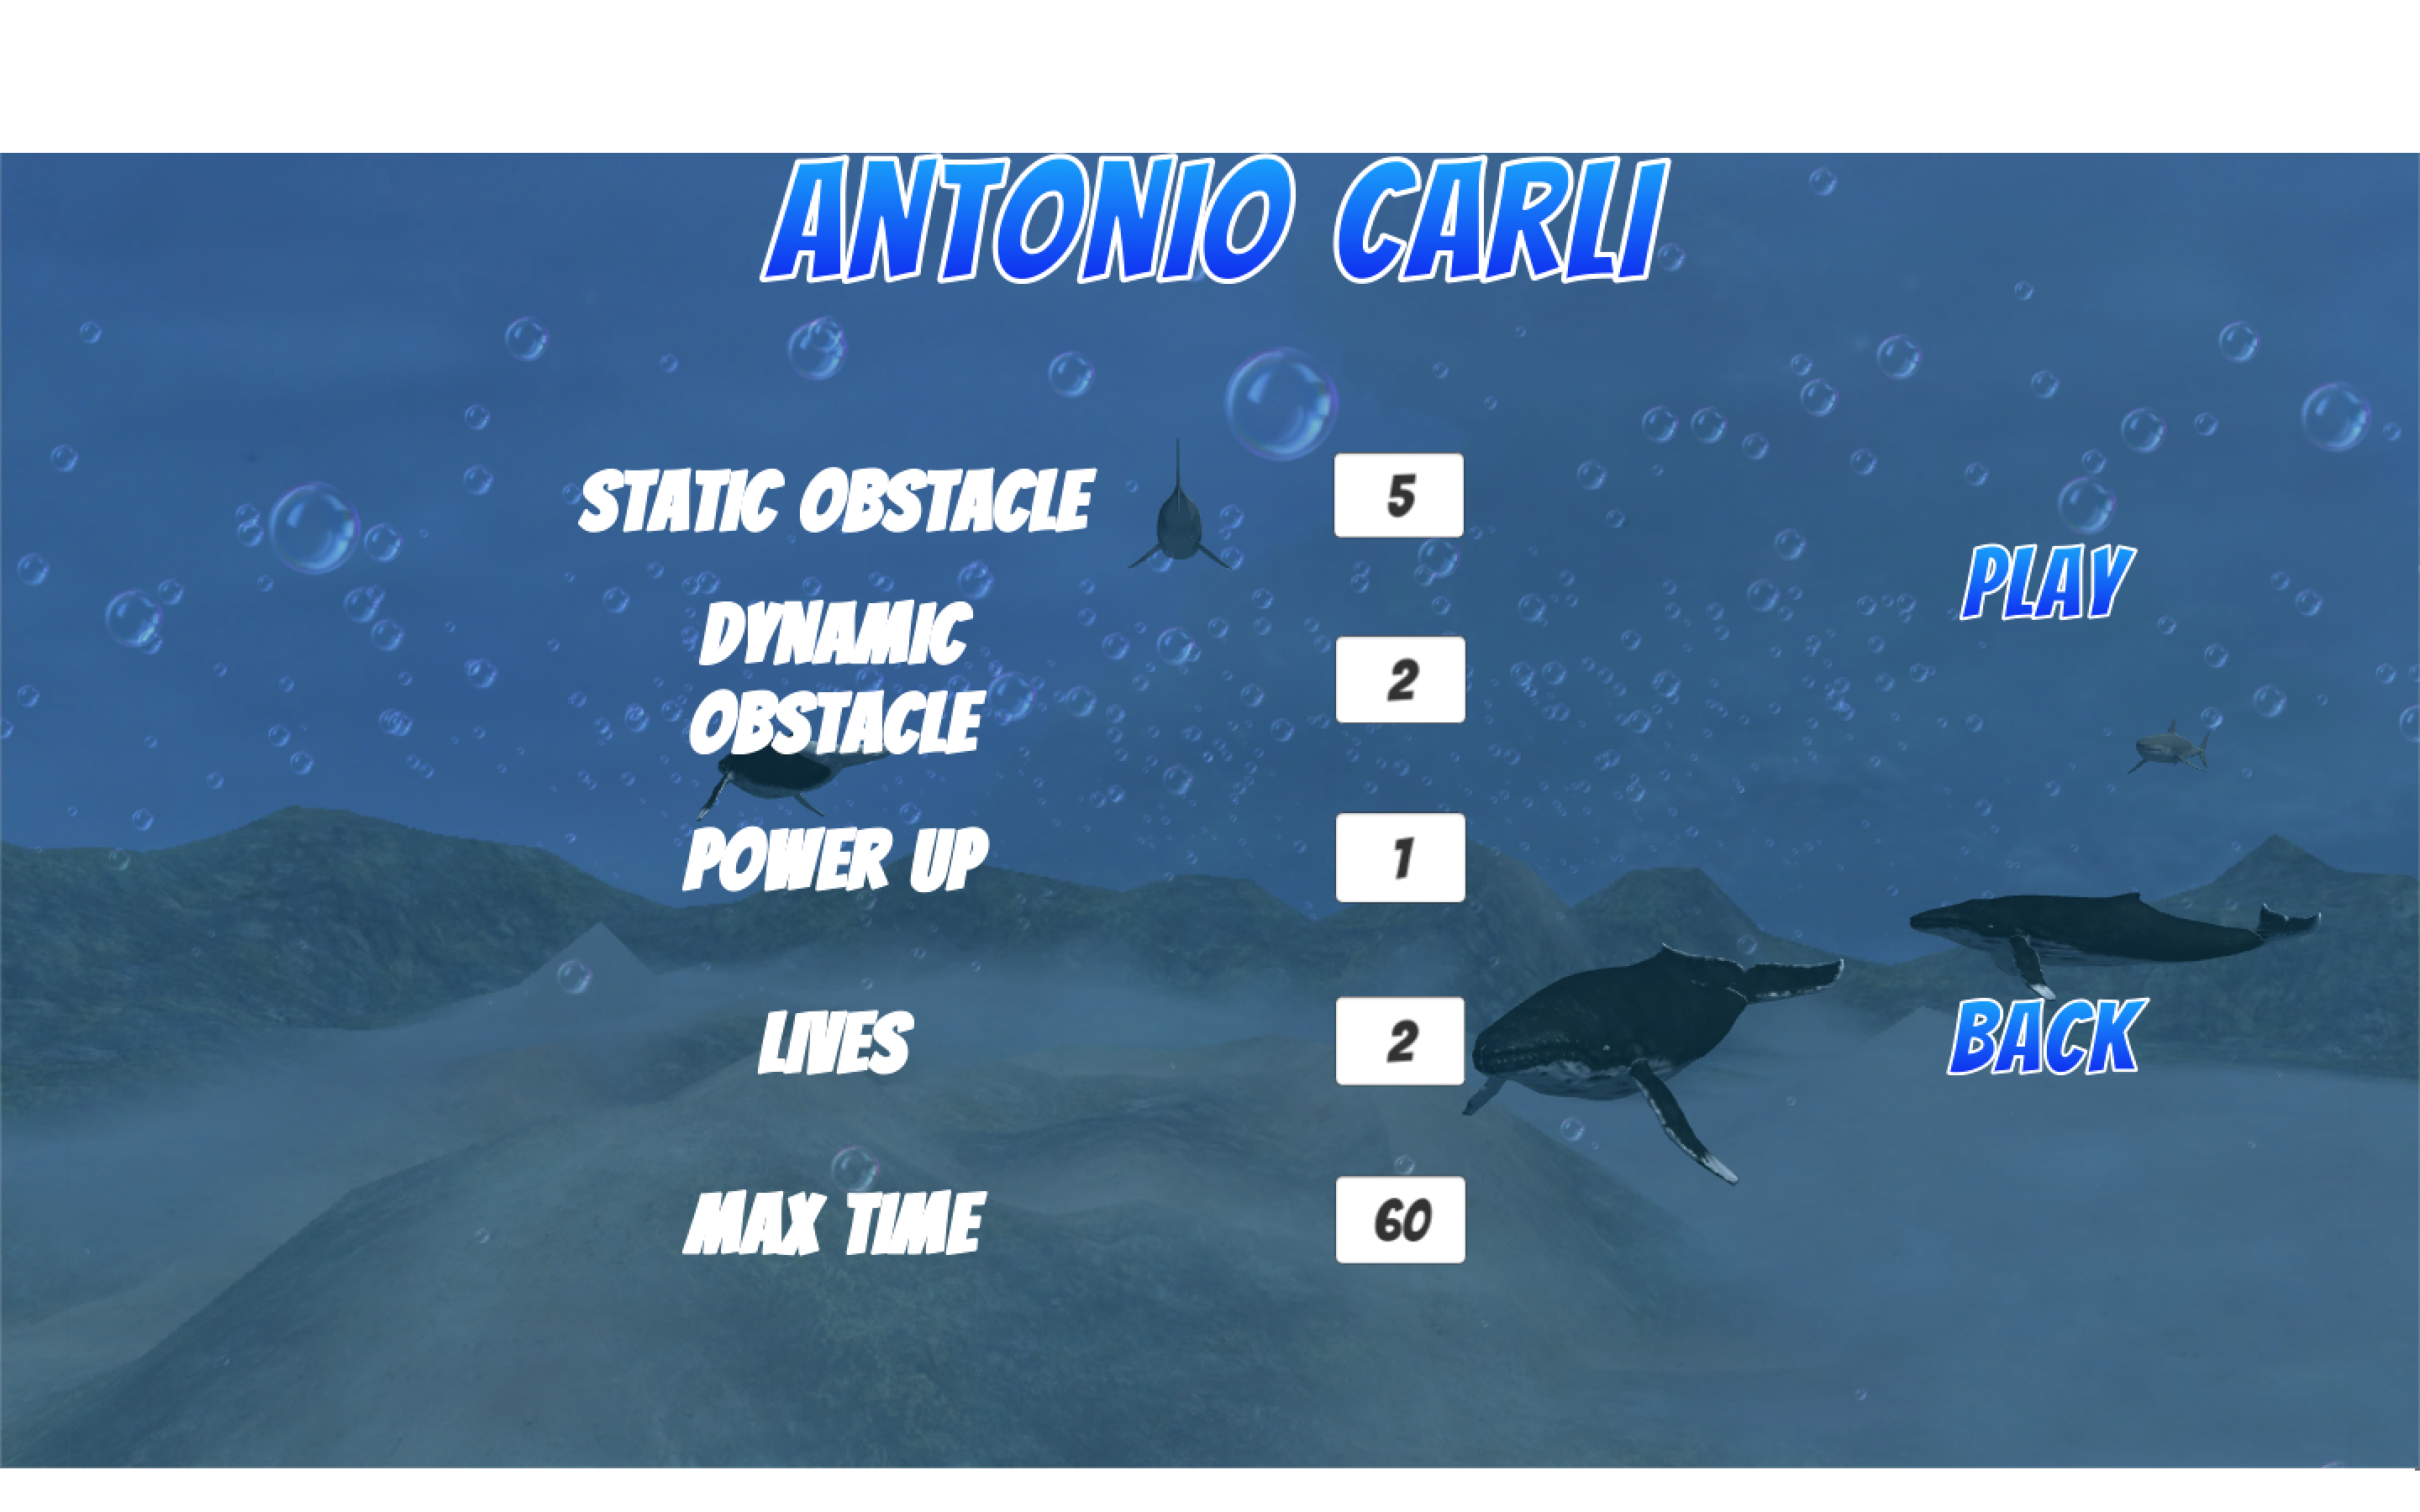
\includegraphics[width=\textwidth]{images/UX/unity/menu/8-runLevelParam}
		\caption{Parameters settings for Dolphin Search }
		\label{fig:unityParamSearch}
	\end{minipage}
\end{figure}

Depending on the selected activity then the user is redirected into the session parameters' page (Figure \ref{fig:unityParamRun}, \ref{fig:unityParamSearch}) where is possible to modify once again the patient's parameters for the next session and to store them permanently.
\pagebreak
\subsubsection{Dolphin Run}
%\begin{figure}[h!]
%	\includegraphics[width=\textwidth]{images/UX/unity/run/1-obstacleAvoid}
%	\caption{Dolphin Run activity}
%	\label{fig:unityObstAvoid}
%\end{figure}
%\begin{figure}[h!]
%	\includegraphics[width=\textwidth]{images/UX/unity/run/1-crossroad}
%	\caption{Example of crossroad and requested interaction in the Dolphin Run}
%	\label{fig:unityDolphRunCross}
%\end{figure}
Once the Dolphin Run activity is selected and one of the two possible levels is chosen the session will start.
This activity consists in an obstacle course during which the patient, interacting with the \textit{Dolphin SAM} smart toy has to control the virtual dolphin in the game in order to proceed.
The interaction for this activity is both full body and tactile: by rotating the \textit{Dolphin SAM} smart toy upwards (by tilting the head upward like in Figure \ref{fig:unityObstAvoid}), downwards (by tilting the head downwards), clockwise (by tilting the right fin towards the ground) and counterclockwise (by tilting the left fin towards the ground) the patient is able to change the proceeding direction of the virtual dolphin respectively to an up direction, a down direction, a right direction and a left direction.

During the course there are multiple obstacle both static and dynamic which density is defined by the parameters set beforehand via the website (Figure \ref{fig:webPatPar1}) or the unity menu (Figure \ref{fig:unityParamRun}). Other than obstacles is also possible to set the maximum time available to finish the level, the number of lives available and the number of power up(%fatti dire quali sono i power up).
 Furthermore there are also crossroads in the levels in which the patient has to use the touch sensors present on the \textit{Dolphin SAM}'s right fin and left fin in order to choose in which direction to proceed (Figure \ref{fig:unityDolphRunCross}).

Once completed the level the activity will terminate and forward the user back to the menu (Figure \ref{fig:unityModSel}).
\subsubsection{Dolphin Search}
After selecting the Dolphin Search game mode and setting the desired parameters of the session (that consists in the number of \textit{Search Zones} to be put into the game and their respective number of starfishes to collect) the Dolphin Search session will start.

In this activity the patient will use multiple interaction schemes that will alternate with the two game phases of the activity:
\begin{itemize}
%	\begin{figure}[h!]
%		\includegraphics[width=\textwidth]{images/UX/unity/search/searchZone}
%		\caption{Represents a \textit{Search Zone} inside the gaming area.}
%		\label{fig:unitySearchZone}
%	\end{figure}
	\item {$ - $} \textbf{Discovery phase} : in which the patient uses the same controls as in the Dolphin Run activity to move around a virtual area in order to find the \textit{Search Zones} (Figure \ref{fig:unitySearchZone}) Notice that differently from the other activity here the patient has to give an input to the system in order to move forward that consist in touching both the left and right fin of the \textit{Dolphin SAM} smart toy. 
	%	\begin{figure}[h!]
	%		\includegraphics[width=\textwidth]{images/UX/unity/search/magnifierRequest}
	%		\caption{Once in a \textit{Search Zone} the magnifier is requested to pass into the search phase}
	%		\label{fig:unityMagnifierRequest}
	%	\end{figure}
	When a \textit{Search Zone} is found the user, in order to proceed to the search phase has to insert into the \textit{Dolphin SAM} mouth the magnifier toy equipped with an RFID (Figure \ref{fig:unityMagnifierRequest}).
	Once scanned by the RFID reader in \textit{Dolphin SAM's} mouth the search phase will start.
%	\begin{figure}[h!]
%		\includegraphics[width=\textwidth]{images/UX/unity/search/magnifierFocus}
%		\caption{The display on the ground shows the magnifier's focus inside the current \textit{Search Zone}}
%		\label{fig:unityMagnifierFocus}
%	\end{figure}
	\item {$ - $} \textbf{Search phase} : during this phase the patient has to find the sea stars, that are hidden below the sand level in the \textit{Search Zone}, by moving around the Magic Room while having the \textit{Search Zone's} seabed projected on the ground. In fact the system tracks the position of the patient inside the magic room using the Kinect and represents it in the virtual environment by using a white disk called the magnifier's focus(Figure \ref{fig:unityMagnifierFocus}).
	%	\begin{figure}[h!]
	%		\includegraphics[width=\textwidth]{images/UX/unity/search/seastarFound}
	%		\caption{The display on the ground shows when a sea star is found}
	%		\label{fig:unityMagnifierSeastar}
	%	\end{figure}
	A sea star is collected when the magnifier's focus passes over it as shown in Figure \ref{fig:unityMagnifierSeastar}. Once all the sea star containsed in a \textit{Search Zone} are found, if there are more \textit{Search Zones} in the map the Discovery phase will resume, otherwise the session will terminate and forward the user back to the main menu (Figure \ref{fig:unityModSel}).
\end{itemize}